
%% bare_conf.tex
%% V1.4a
%% 2014/09/17
%% by Michael Shell
%% See:
%% http://www.michaelshell.org/
%% for current contact information.
%%
%% This is a skeleton file demonstrating the use of IEEEtran.cls
%% (requires IEEEtran.cls version 1.8a or later) with an IEEE
%% conference paper.
%%
%% Support sites:
%% http://www.michaelshell.org/tex/ieeetran/
%% http://www.ctan.org/tex-archive/macros/latex/contrib/IEEEtran/
%% and
%% http://www.ieee.org/

%%*************************************************************************
%% Legal Notice:
%% This code is offered as-is without any warranty either expressed or
%% implied; without even the implied warranty of MERCHANTABILITY or
%% FITNESS FOR A PARTICULAR PURPOSE! 
%% User assumes all risk.
%% In no event shall IEEE or any contributor to this code be liable for
%% any damages or losses, including, but not limited to, incidental,
%% consequential, or any other damages, resulting from the use or misuse
%% of any information contained here.
%%
%% All comments are the opinions of their respective authors and are not
%% necessarily endorsed by the IEEE.
%%
%% This work is distributed under the LaTeX Project Public License (LPPL)
%% ( http://www.latex-project.org/ ) version 1.3, and may be freely used,
%% distributed and modified. A copy of the LPPL, version 1.3, is included
%% in the base LaTeX documentation of all distributions of LaTeX released
%% 2003/12/01 or later.
%% Retain all contribution notices and credits.
%% ** Modified files should be clearly indicated as such, including  **
%% ** renaming them and changing author support contact information. **
%%
%% File list of work: IEEEtran.cls, IEEEtran_HOWTO.pdf, bare_adv.tex,
%%                    bare_conf.tex, bare_jrnl.tex, bare_conf_compsoc.tex,
%%                    bare_jrnl_compsoc.tex, bare_jrnl_transmag.tex
%%*************************************************************************


% *** Authors should verify (and, if needed, correct) their LaTeX system  ***
% *** with the testflow diagnostic prior to trusting their LaTeX platform ***
% *** with production work. IEEE's font choices and paper sizes can       ***
% *** trigger bugs that do not appear when using other class files.       ***                          ***
% The testflow support page is at:
% http://www.michaelshell.org/tex/testflow/



\documentclass[conference]{IEEEtran}
\usepackage{appendix}
\usepackage{listings}
\usepackage{pdfpages}
\usepackage{hyperref}
\usepackage[
backend=biber,
style=ieee,
]{biblatex}
\addbibresource{bib.bib}
% Some Computer Society conferences also require the compsoc mode option,
% but others use the standard conference format.
%
% If IEEEtran.cls has not been installed into the LaTeX system files,
% manually specify the path to it like:
% \documentclass[conference]{../sty/IEEEtran}





% Some very useful LaTeX packages include:
% (uncomment the ones you want to load)


% *** MISC UTILITY PACKAGES ***
%
%\usepackage{ifpdf}
% Heiko Oberdiek's ifpdf.sty is very useful if you need conditional
% compilation based on whether the output is pdf or dvi.
% usage:
% \ifpdf
%   % pdf code
% \else
%   % dvi code
% \fi
% The latest version of ifpdf.sty can be obtained from:
% http://www.ctan.org/tex-archive/macros/latex/contrib/oberdiek/
% Also, note that IEEEtran.cls V1.7 and later provides a builtin
% \ifCLASSINFOpdf conditional that works the same way.
% When switching from latex to pdflatex and vice-versa, the compiler may
% have to be run twice to clear warning/error messages.






% *** CITATION PACKAGES ***
%
%\usepackage{cite}
% cite.sty was written by Donald Arseneau
% V1.6 and later of IEEEtran pre-defines the format of the cite.sty package
% \cite{} output to follow that of IEEE. Loading the cite package will
% result in citation numbers being automatically sorted and properly
% "compressed/ranged". e.g., [1], [9], [2], [7], [5], [6] without using
% cite.sty will become [1], [2], [5]--[7], [9] using cite.sty. cite.sty's
% \cite will automatically add leading space, if needed. Use cite.sty's
% noadjust option (cite.sty V3.8 and later) if you want to turn this off
% such as if a citation ever needs to be enclosed in parenthesis.
% cite.sty is already installed on most LaTeX systems. Be sure and use
% version 5.0 (2009-03-20) and later if using hyperref.sty.
% The latest version can be obtained at:
% http://www.ctan.org/tex-archive/macros/latex/contrib/cite/
% The documentation is contained in the cite.sty file itself.






% *** GRAPHICS RELATED PACKAGES ***
%
\usepackage[pdftex]{graphicx}
  % declare the path(s) where your graphic files are
  % \graphicspath{{../pdf/}{../jpeg/}}
  % and their extensions so you won't have to specify these with
  % every instance of \includegraphics
  % \DeclareGraphicsExtensions{.pdf,.jpeg,.png}
% graphicx was written by David Carlisle and Sebastian Rahtz. It is
% required if you want graphics, photos, etc. graphicx.sty is already
% installed on most LaTeX systems. The latest version and documentation
% can be obtained at: 
% http://www.ctan.org/tex-archive/macros/latex/required/graphics/
% Another good source of documentation is "Using Imported Graphics in
% LaTeX2e" by Keith Reckdahl which can be found at:
% http://www.ctan.org/tex-archive/info/epslatex/
%
% latex, and pdflatex in dvi mode, support graphics in encapsulated
% postscript (.eps) format. pdflatex in pdf mode supports graphics
% in .pdf, .jpeg, .png and .mps (metapost) formats. Users should ensure
% that all non-photo figures use a vector format (.eps, .pdf, .mps) and
% not a bitmapped formats (.jpeg, .png). IEEE frowns on bitmapped formats
% which can result in "jaggedy"/blurry rendering of lines and letters as
% well as large increases in file sizes.
%
% You can find documentation about the pdfTeX application at:
% http://www.tug.org/applications/pdftex



% *** MATH PACKAGES ***
%
%\usepackage[cmex10]{amsmath}
% A popular package from the American Mathematical Society that provides
% many useful and powerful commands for dealing with mathematics. If using
% it, be sure to load this package with the cmex10 option to ensure that
% only type 1 fonts will utilized at all point sizes. Without this option,
% it is possible that some math symbols, particularly those within
% footnotes, will be rendered in bitmap form which will result in a
% document that can not be IEEE Xplore compliant!
%
% Also, note that the amsmath package sets \interdisplaylinepenalty to 10000
% thus preventing page breaks from occurring within multiline equations. Use:
%\interdisplaylinepenalty=2500
% after loading amsmath to restore such page breaks as IEEEtran.cls normally
% does. amsmath.sty is already installed on most LaTeX systems. The latest
% version and documentation can be obtained at:
% http://www.ctan.org/tex-archive/macros/latex/required/amslatex/math/





% *** SPECIALIZED LIST PACKAGES ***
%
%\usepackage{algorithmic}
% algorithmic.sty was written by Peter Williams and Rogerio Brito.
% This package provides an algorithmic environment fo describing algorithms.
% You can use the algorithmic environment in-text or within a figure
% environment to provide for a floating algorithm. Do NOT use the algorithm
% floating environment provided by algorithm.sty (by the same authors) or
% algorithm2e.sty (by Christophe Fiorio) as IEEE does not use dedicated
% algorithm float types and packages that provide these will not provide
% correct IEEE style captions. The latest version and documentation of
% algorithmic.sty can be obtained at:
% http://www.ctan.org/tex-archive/macros/latex/contrib/algorithms/
% There is also a support site at:
% http://algorithms.berlios.de/index.html
% Also of interest may be the (relatively newer and more customizable)
% algorithmicx.sty package by Szasz Janos:
% http://www.ctan.org/tex-archive/macros/latex/contrib/algorithmicx/




% *** ALIGNMENT PACKAGES ***
%
%\usepackage{array}
% Frank Mittelbach's and David Carlisle's array.sty patches and improves
% the standard LaTeX2e array and tabular environments to provide better
% appearance and additional user controls. As the default LaTeX2e table
% generation code is lacking to the point of almost being broken with
% respect to the quality of the end results, all users are strongly
% advised to use an enhanced (at the very least that provided by array.sty)
% set of table tools. array.sty is already installed on most systems. The
% latest version and documentation can be obtained at:
% http://www.ctan.org/tex-archive/macros/latex/required/tools/


% IEEEtran contains the IEEEeqnarray family of commands that can be used to
% generate multiline equations as well as matrices, tables, etc., of high
% quality.




% *** SUBFIGURE PACKAGES ***
%\ifCLASSOPTIONcompsoc
%  \usepackage[caption=false,font=normalsize,labelfont=sf,textfont=sf]{subfig}
%\else
%  \usepackage[caption=false,font=footnotesize]{subfig}
%\fi
% subfig.sty, written by Steven Douglas Cochran, is the modern replacement
% for subfigure.sty, the latter of which is no longer maintained and is
% incompatible with some LaTeX packages including fixltx2e. However,
% subfig.sty requires and automatically loads Axel Sommerfeldt's caption.sty
% which will override IEEEtran.cls' handling of captions and this will result
% in non-IEEE style figure/table captions. To prevent this problem, be sure
% and invoke subfig.sty's "caption=false" package option (available since
% subfig.sty version 1.3, 2005/06/28) as this is will preserve IEEEtran.cls
% handling of captions.
% Note that the Computer Society format requires a larger sans serif font
% than the serif footnote size font used in traditional IEEE formatting
% and thus the need to invoke different subfig.sty package options depending
% on whether compsoc mode has been enabled.
%
% The latest version and documentation of subfig.sty can be obtained at:
% http://www.ctan.org/tex-archive/macros/latex/contrib/subfig/




% *** FLOAT PACKAGES ***
%
%\usepackage{fixltx2e}
% fixltx2e, the successor to the earlier fix2col.sty, was written by
% Frank Mittelbach and David Carlisle. This package corrects a few problems
% in the LaTeX2e kernel, the most notable of which is that in current
% LaTeX2e releases, the ordering of single and double column floats is not
% guaranteed to be preserved. Thus, an unpatched LaTeX2e can allow a
% single column figure to be placed prior to an earlier double column
% figure. The latest version and documentation can be found at:
% http://www.ctan.org/tex-archive/macros/latex/base/


%\usepackage{stfloats}
% stfloats.sty was written by Sigitas Tolusis. This package gives LaTeX2e
% the ability to do double column floats at the bottom of the page as well
% as the top. (e.g., "\begin{figure*}[!b]" is not normally possible in
% LaTeX2e). It also provides a command:
%\fnbelowfloat
% to enable the placement of footnotes below bottom floats (the standard
% LaTeX2e kernel puts them above bottom floats). This is an invasive package
% which rewrites many portions of the LaTeX2e float routines. It may not work
% with other packages that modify the LaTeX2e float routines. The latest
% version and documentation can be obtained at:
% http://www.ctan.org/tex-archive/macros/latex/contrib/sttools/
% Do not use the stfloats baselinefloat ability as IEEE does not allow
% \baselineskip to stretch. Authors submitting work to the IEEE should note
% that IEEE rarely uses double column equations and that authors should try
% to avoid such use. Do not be tempted to use the cuted.sty or midfloat.sty
% packages (also by Sigitas Tolusis) as IEEE does not format its papers in
% such ways.
% Do not attempt to use stfloats with fixltx2e as they are incompatible.
% Instead, use Morten Hogholm'a dblfloatfix which combines the features
% of both fixltx2e and stfloats:
%
% \usepackage{dblfloatfix}
% The latest version can be found at:
% http://www.ctan.org/tex-archive/macros/latex/contrib/dblfloatfix/




% *** PDF, URL AND HYPERLINK PACKAGES ***
%
%\usepackage{url}
% url.sty was written by Donald Arseneau. It provides better support for
% handling and breaking URLs. url.sty is already installed on most LaTeX
% systems. The latest version and documentation can be obtained at:
% http://www.ctan.org/tex-archive/macros/latex/contrib/url/
% Basically, \url{my_url_here}.




% *** Do not adjust lengths that control margins, column widths, etc. ***
% *** Do not use packages that alter fonts (such as pslatex).         ***
% There should be no need to do such things with IEEEtran.cls V1.6 and later.
% (Unless specifically asked to do so by the journal or conference you plan
% to submit to, of course. )


% correct bad hyphenation here
\hyphenation{op-tical net-works semi-conduc-tor}


\begin{document}
%
% paper title
% Titles are generally capitalized except for words such as a, an, and, as,
% at, but, by, for, in, nor, of, on, or, the, to and up, which are usually
% not capitalized unless they are the first or last word of the title.
% Linebreaks \\ can be used within to get better formatting as desired.
% Do not put math or special symbols in the title.
\title{A Mandatory: Strandbeest}


% author names and affiliations
% use a multiple column layout for up to three different
% affiliations
\author{\IEEEauthorblockN{Amanda Bak Christensen}
\IEEEauthorblockA{ambc@itu.dk}
\and
\IEEEauthorblockN{Tore Asbjørn Tonnisen Kjelds}
\IEEEauthorblockA{tokj@itu.dk}
\and
\IEEEauthorblockN{Stefan Krummenacher}
\IEEEauthorblockA{skru@itu.dk}}

% conference papers do not typically use \thanks and this command
% is locked out in conference mode. If really needed, such as for
% the acknowledgment of grants, issue a \IEEEoverridecommandlockouts
% after \documentclass

% for over three affiliations, or if they all won't fit within the width
% of the page, use this alternative format:
% 
%\author{\IEEEauthorblockN{Michael Shell\IEEEauthorrefmark{1},
%Homer Simpson\IEEEauthorrefmark{2},
%James Kirk\IEEEauthorrefmark{3}, 
%Montgomery Scott\IEEEauthorrefmark{3} and
%Eldon Tyrell\IEEEauthorrefmark{4}}
%\IEEEauthorblockA{\IEEEauthorrefmark{1}School of Electrical and Computer Engineering\\
%Georgia Institute of Technology,
%Atlanta, Georgia 30332--0250\\ Email: see http://www.michaelshell.org/contact.html}
%\IEEEauthorblockA{\IEEEauthorrefmark{2}Twentieth Century Fox, Springfield, USA\\
%Email: homer@thesimpsons.com}
%\IEEEauthorblockA{\IEEEauthorrefmark{3}Starfleet Academy, San Francisco, California 96678-2391\\
%Telephone: (800) 555--1212, Fax: (888) 555--1212}
%\IEEEauthorblockA{\IEEEauthorrefmark{4}Tyrell Inc., 123 Replicant Street, Los Angeles, California 90210--4321}}




% use for special paper notices
\IEEEspecialpapernotice{Course code: KSHOMAA1KU\\28th of May 2025}




% make the title area
\maketitle

% For peer review papers, you can put extra information on the cover
% page as needed:
% \ifCLASSOPTIONpeerreview
% \begin{center} \bfseries EDICS Category: 3-BBND \end{center}
% \fi
%
% For peerreview papers, this IEEEtran command inserts a page break and
% creates the second title. It will be ignored for other modes.
\IEEEpeerreviewmaketitle
\newpage 

%INSERT SECTIONS HERE
\newpage
\section{Introduction}
The motivation behind this project was to build a mobile robot capable of walking across various ground surfaces, combining both mechanical movement and wireless control. Unlike wheeled robots, a legged design can adapt more easily to uneven or soft terrain, making it more able to move in real-world environments. We also introduce a further addition in making the robot controllable in real time via a Bluetooth connection to an app. The finished robot can be seen in figure: \ref{fig:robot}

\section{Background}
The concept of using mechanical linkages to create walking robots is not new. The Theo Jansen linkage, originally designed by kinetic artist Theo Jansen for wind-powered sculptures called "Strandbeests", has been used in previous robotics research with a focus on gait analysis \cite{nansai2013dynamicanalysis} \cite{hernandez2016homemade} for its ability to generate smooth, lifelike walking motion using a single rotary actuator. 

Projects similar to this has been done, an example being \cite{jeremySCook}, in which a premade Strandbeest kit was adapted to be remote controlled. In addition, previous work has also been done using the ultrasonic sensor for obstacle detection. But, to the best of our knowledge no one has combined both obstacle detection, remote controllability and OEM parts. 

Other additions as actuated feet on the legs to increase traction, and a modular design that making it easier to extend the number of legs. 

\section{Requirements}
To meet the project goals, the robot was designed with the following requirements:

\begin{itemize}
    \item  The robot must use Theo Jansen-style mechanical linkages for walking, powered by two DC motors.
    \item The robot must support Bluetooth control via a mobile app, allowing the user to steer and adjust speed remotely.
    \item  An ultrasonic distance sensor must detect obstacles and trigger braking.
    \item The robot must operate on battery power to ensure mobility.
    \item The design should support easy extension of the number of legs, with a mechanical structure that allows scaling.
    \item Legs must be fitted with actuated feet to increase grip and reduce slipping on smooth surfaces.
    \item The robot should be able to move reliably on a variety of surfaces.
\end{itemize}

\begin{figure}[!htb]
    \centering
    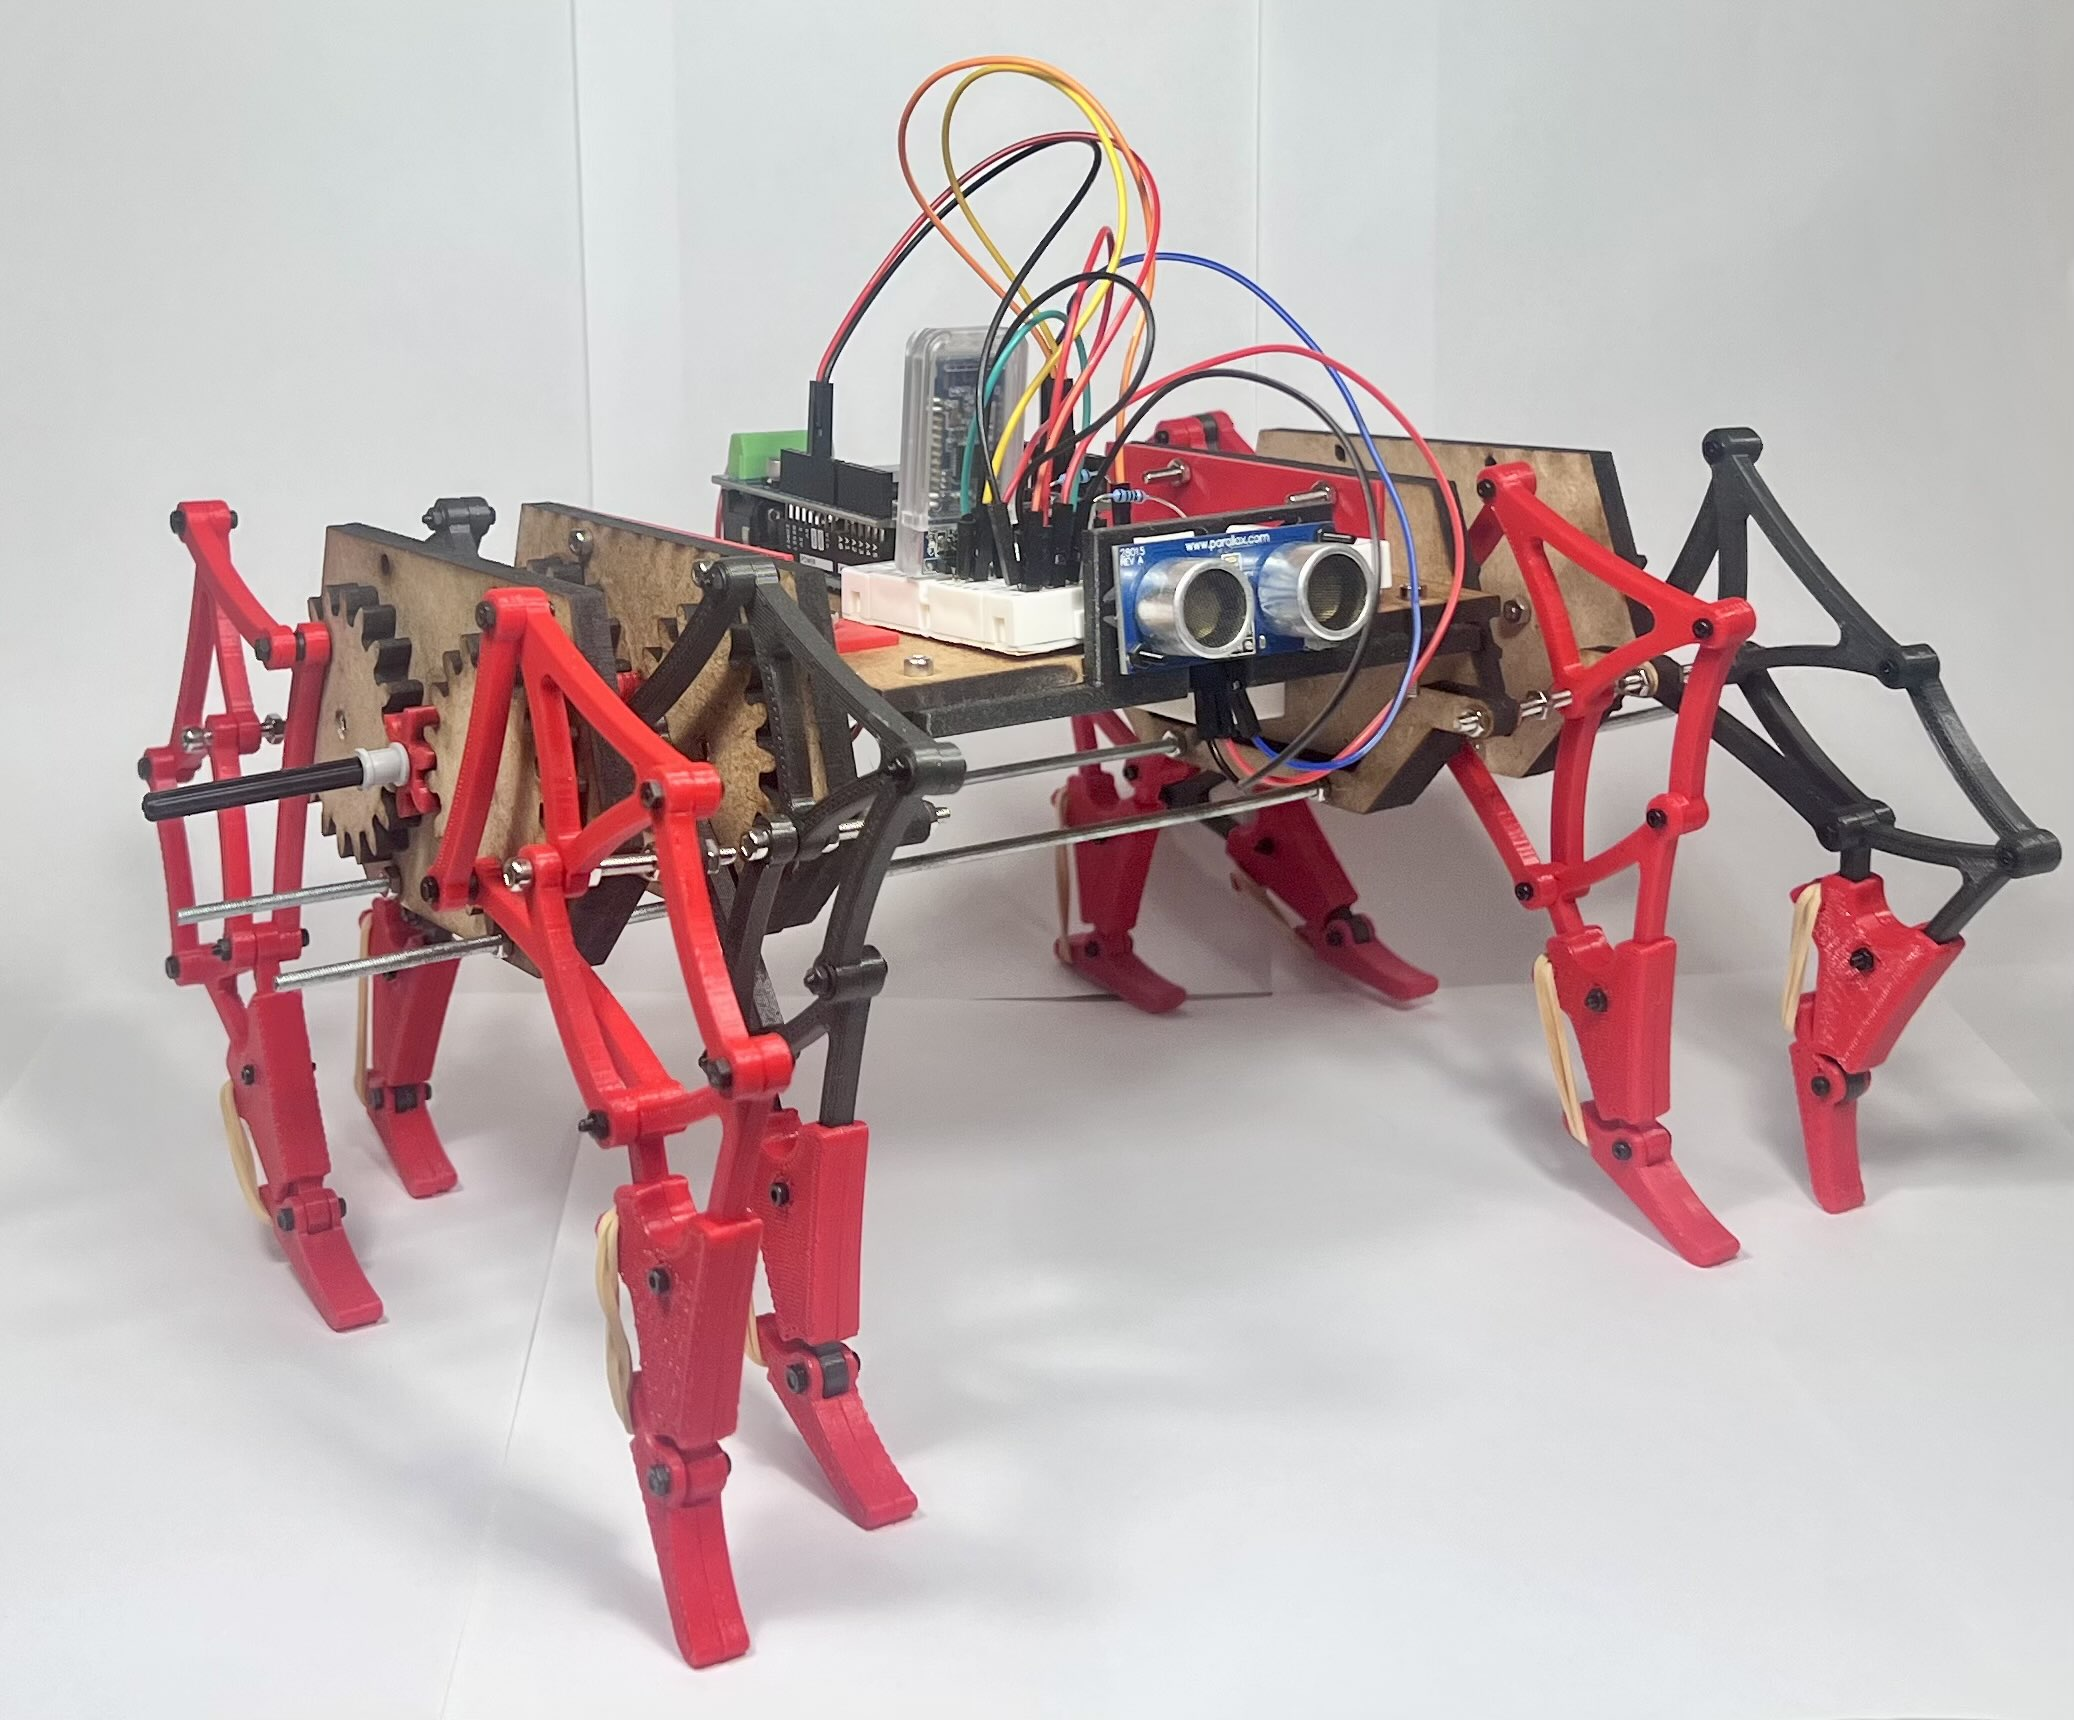
\includegraphics[width=1\linewidth]{images/Roboty.jpg}
    \caption{Assembled robot}
    \label{fig:robot}
\end{figure}

\section{Description}
%How does your device work? Describe in as much detail as you can fit into the report. It should contain three subsections: Mechanics, Electronics and software/Firmware. Describe also what alternatives you analyzed for the different parts of your device. Why did you select the alternative that you finally used?


This section covers a description of the robot, along with potential consderations for alternatives wihtin each decision.
\subsection{Mechanics}
During the design proces of the project it was identified that the main obstacle would be friction. As such many design choices came down to minimizing that factor. 
\subsubsection{Base-plate}
The base plate is where most of the components are located. The base plate is designed for mounting components on either side, as to reduce the overall size, thereby lowering the weight of the robot. Two Dc-motors are mounted on the bottom side along with the ultrasound sensor holder. The mounting mechanism for the DC-motors are self designed holders that screw in through the botom of the plate. The same holes are used on the top side of plate to mount L-shaped brackets that are used to fasten the leg mounting plate to the base-plate. A slot is cut-out on the rear of the baseplate, is used for cable management of the DC-motor wires that are connected to the arduino, this was done minimize the chance fot he wires being tangled in any of the gears. The arduino and breadboard are both mounted on the top-side of the baseplate. The arduino is mounted with screws through the base plate, and the breadboard is mounted with double sided tape that was already applied. The baseplates materials is 4mm MDF, that was cut out using a laser cutter. \\
\begin{figure} [!htb]
    \centering
    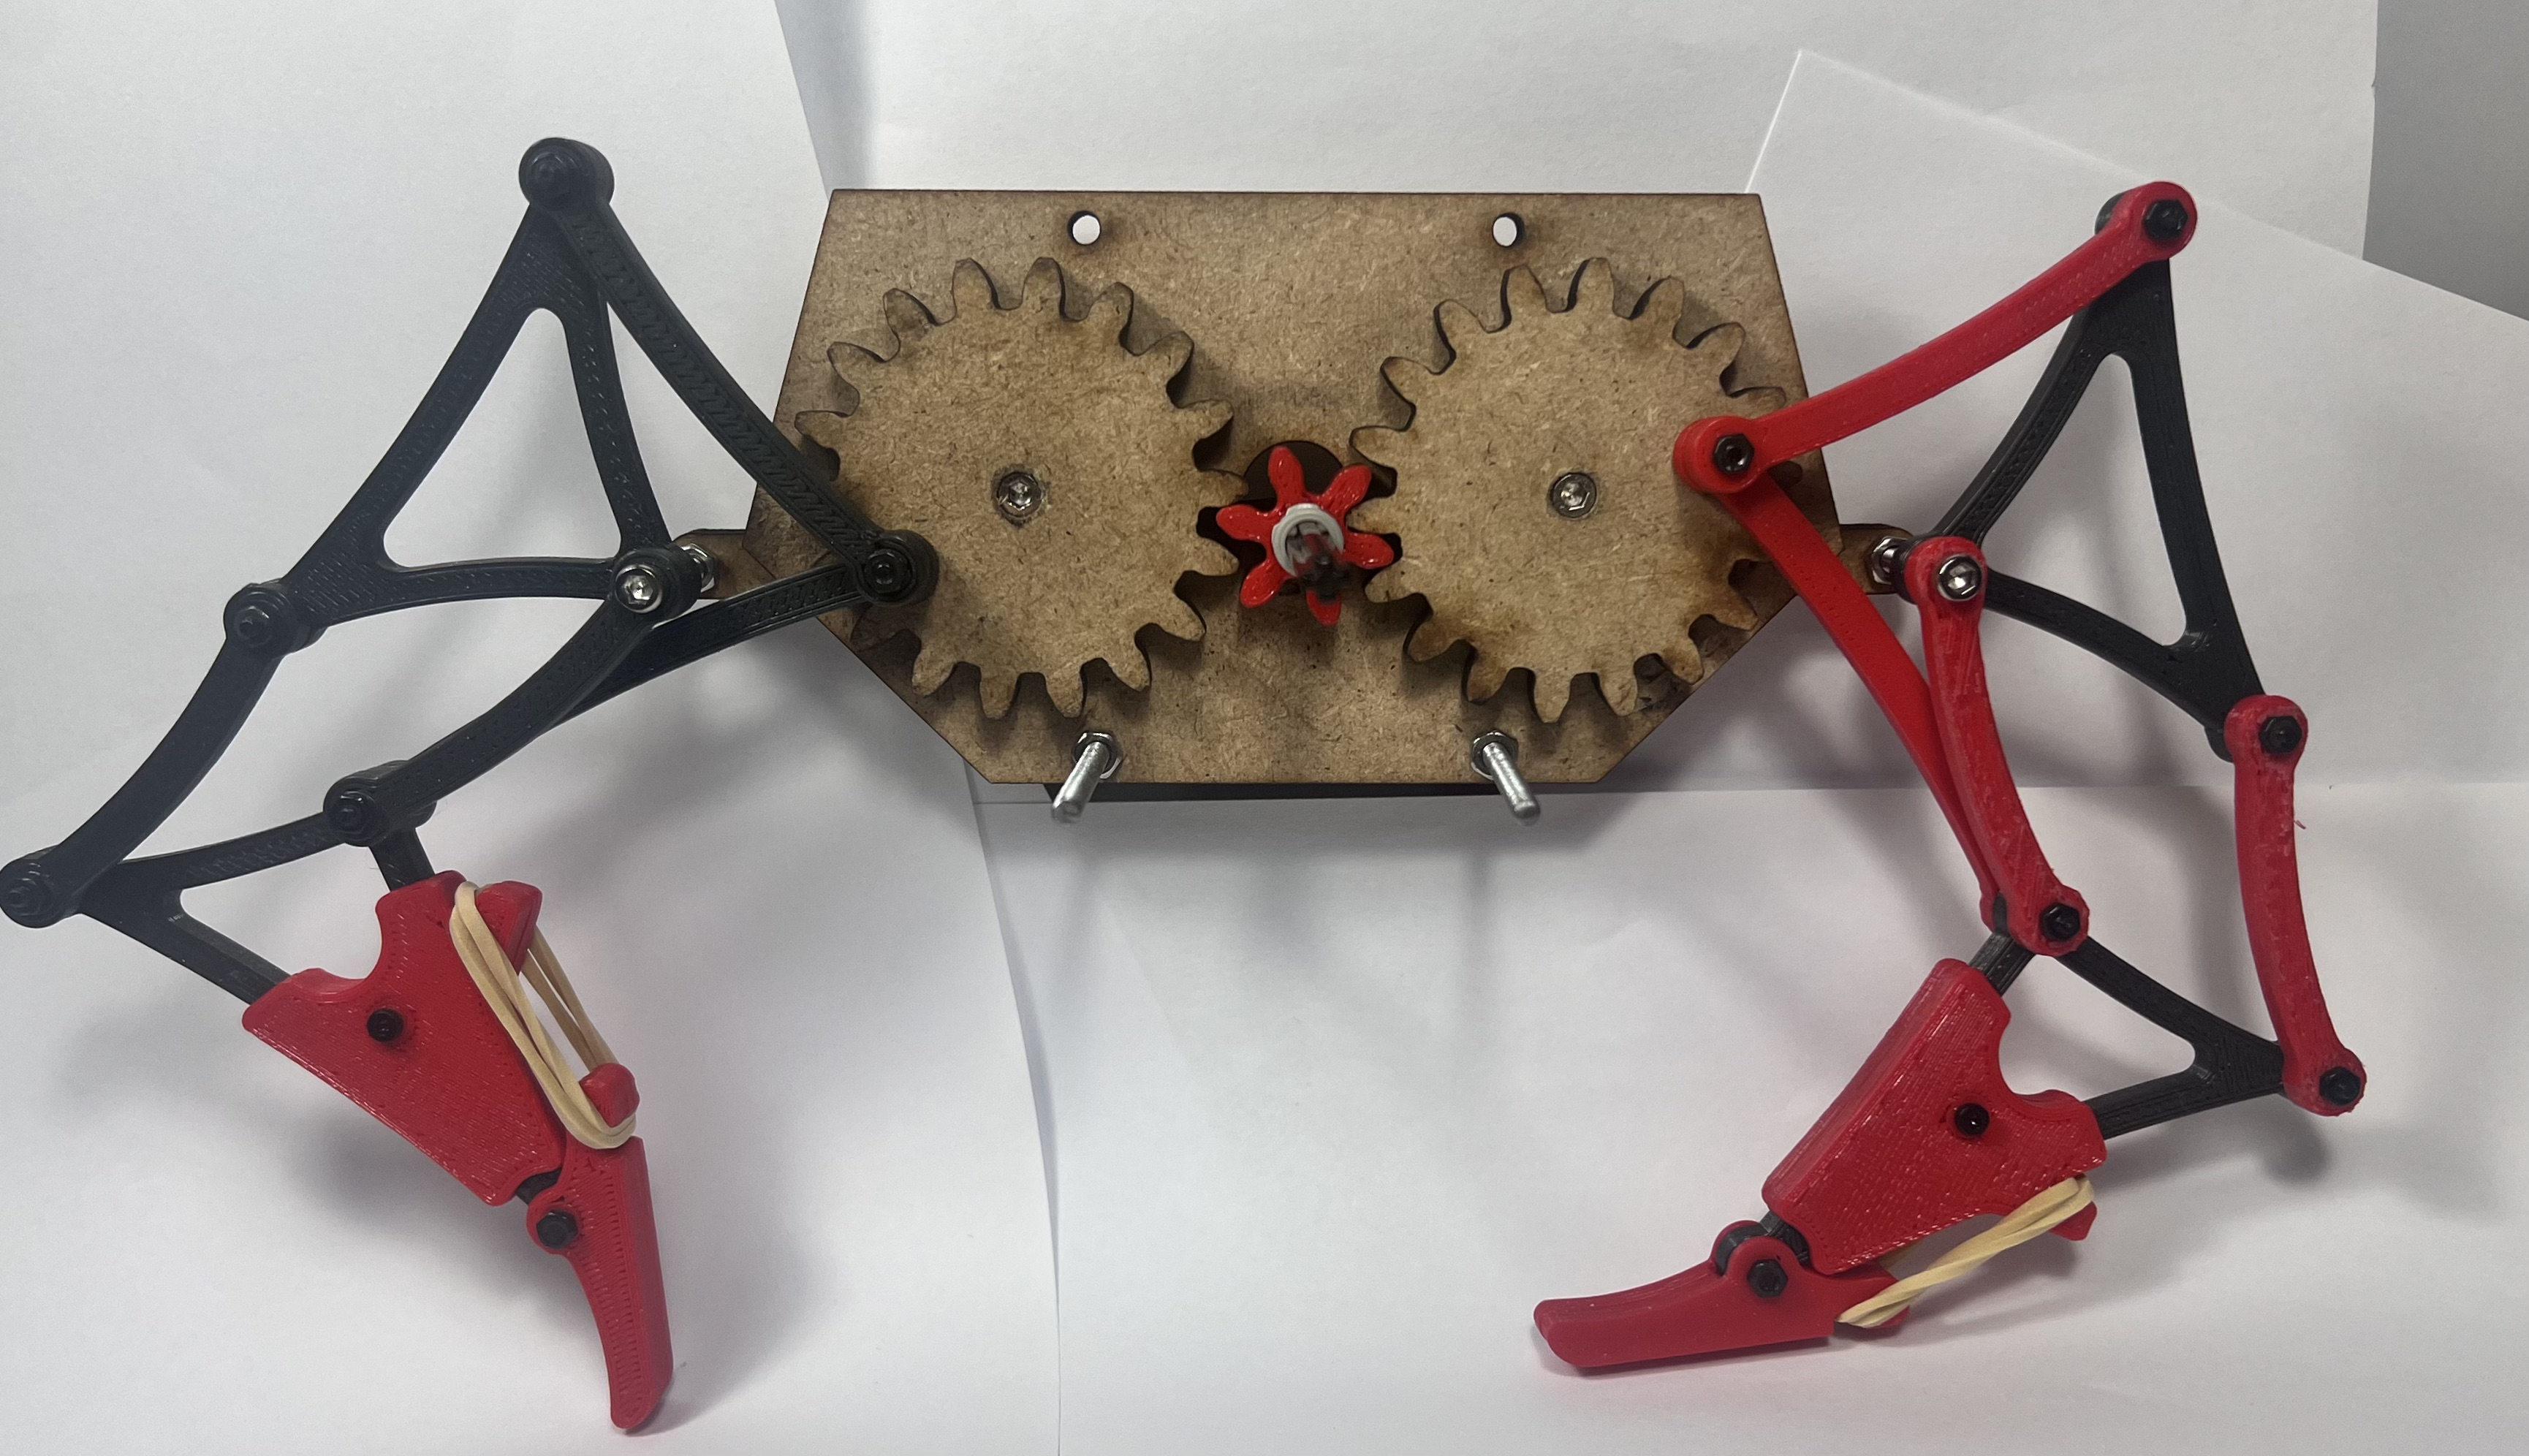
\includegraphics[width=1\linewidth]{images/LMA.jpeg}       
    \caption{Fully assembled leg mounting plate}
    \label{fig:leg_mount_plate}
\end{figure}
\subsubsection{Leg-mounting-plate}
The leg-mounting plate is attached to the base plate using a custom-designed L-bracket and serves as the mounting point for both the gears and legs. A central hole with a 12mm diameter is cut into the middle of the plate, accommodating the rotating central axle. On either side of this hole, two gears are mounted, which connect to the Theo Jansen linkages. These gears operate in a 1:3 ratio, effectively reducing the torque required from the motors. A 1:1 gear ratio was tested during development but was found to demand excessive torque, allowing movement only at the motors' maximum PWM setting. With the 1:3 gear ratio, movement—though slower—was achievable even at a PWM setting of 135.
\\ \\
A bracket is mounted on the back of the plate to secure one of the Theo Jansen joints in place. The primary design goal was to make the leg-mounting plate modular, enabling additional plates to be easily attached to either side. This was accomplished with two holes at the bottom of the plate where two 3mm metal rods can be inserted, and fastened with bolts, serving both as mounting points and alignment guides. The plate, was cut out of 6mm MDF, using a laser cutter. The thicker MDF was chosen because of the increased stress that these plates would incur. A fully assembled Leg-mounting-plate can be seen in figure: \ref{fig:leg_mount_plate}
\\
\subsubsection{Theo-jansen linkage}
The main mechanism of the robot is the Theo Jansen linkage, which acts as the legs. This type of linkage is a planar system with a single degree of freedom, meaning it can be driven by just one rotary input. When the central link is powered by a motor, it moves the rest of the connected links in a coordinated way, creating a smooth, walking motion that mimics a natural gait.
\\ \\
\begin{figure} [!htb]
    \centering
    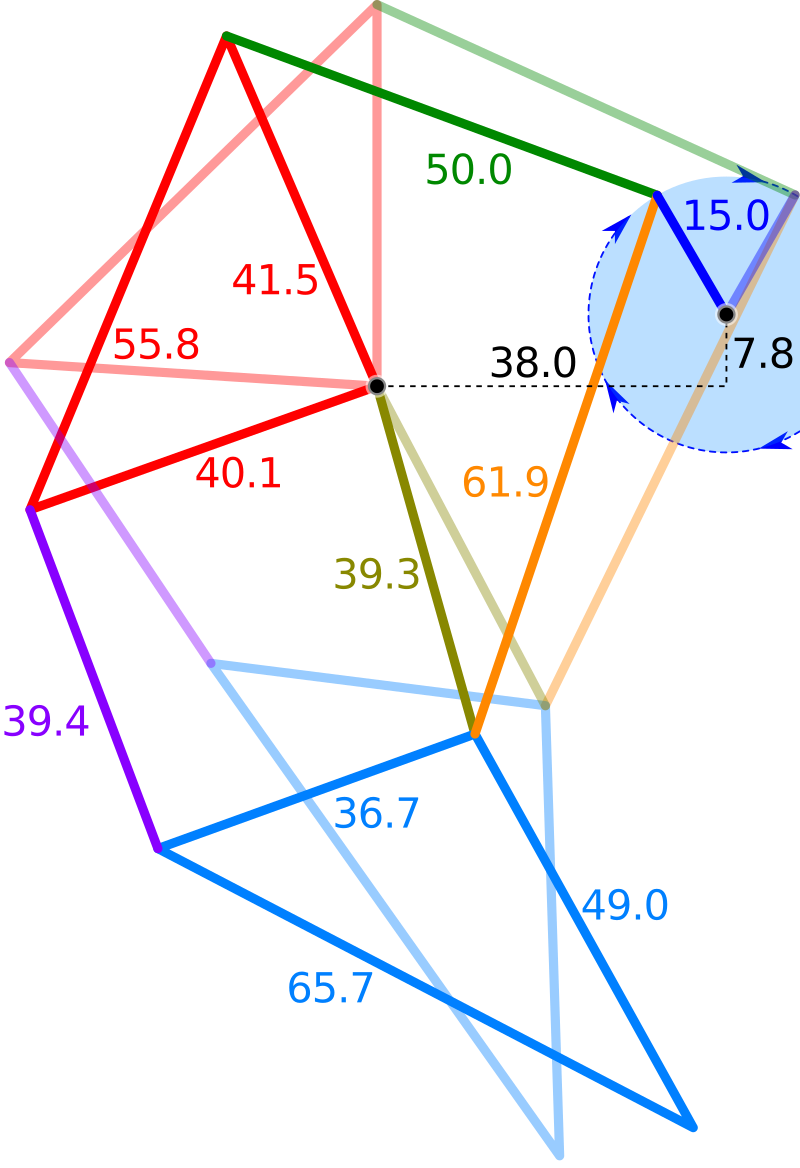
\includegraphics[width=1\linewidth]{images/Jansen's_Linkage.svg.png}
    \caption{Dimensions of the Theo Jansen linkage\cite{jansen2016strandbeest}}
    \label{fig:jansen_dimension}
\end{figure}
The linkage components are connected using revolute joints, which limit movement to rotation only. The leg design is based on common Theo Jansen dimensions (see figure: \ref{fig:jansen_dimension}. Two DC motors are used to drive the legs. Each motor is connected to a gear that turns the central linkage, powering the gear that turns the linkages. The gears, as mentioned above is set to a 1:3 gear ratio. The main joint of the linkage is attached to gear, while another joint is fixed in place using the bracket on the back of the Leg-mounting-plate. All other joints can move freely. Then, when the gear turns, the legs move in a natural gait. 
\\ \\
The main challenge in getting the Theo Jansen linkages to move smoothly is friction. Because of the downward pressure applied at each joint, significant resistance builds up, making motion less efficient. An additional source of friction comes from the contact between two linkages rubbing against each other within the joint. To reduce this effect, we experimented with different materials to determine which offered the lowest friction during movement. we tested two different materials for the linkage components: laser-cut MDF and 3D-printed PLA. The PLA parts resulted in noticeably less friction, allowing us to reduce the required PWM setting by 15 compared to the MDF version. We believe this improvement is because of the reduced surface contact area and smoother finish of the 3D-printed PLA components. \\
\subsubsection{Actuated feet}
In an attempt to increase stability and mobility on uneven terrain, the robot is equipped with actuated feet consisting of two components: a foot and a boot (figure: \ref{fig:feet}). These parts are designed as a clamshell that wraps around the lower leg segment and is secured using a single bolt and nut. A rubber band is attached from the heel of the foot to the boot, providing a passive return force that helps keep the foot in contact with the ground during motion. We found this setup to improve traction and energy transfer, allowing the robot to move on rougher surfaces and increasing the overall forward walking speed.
\begin{figure} [!htb]
    \centering
    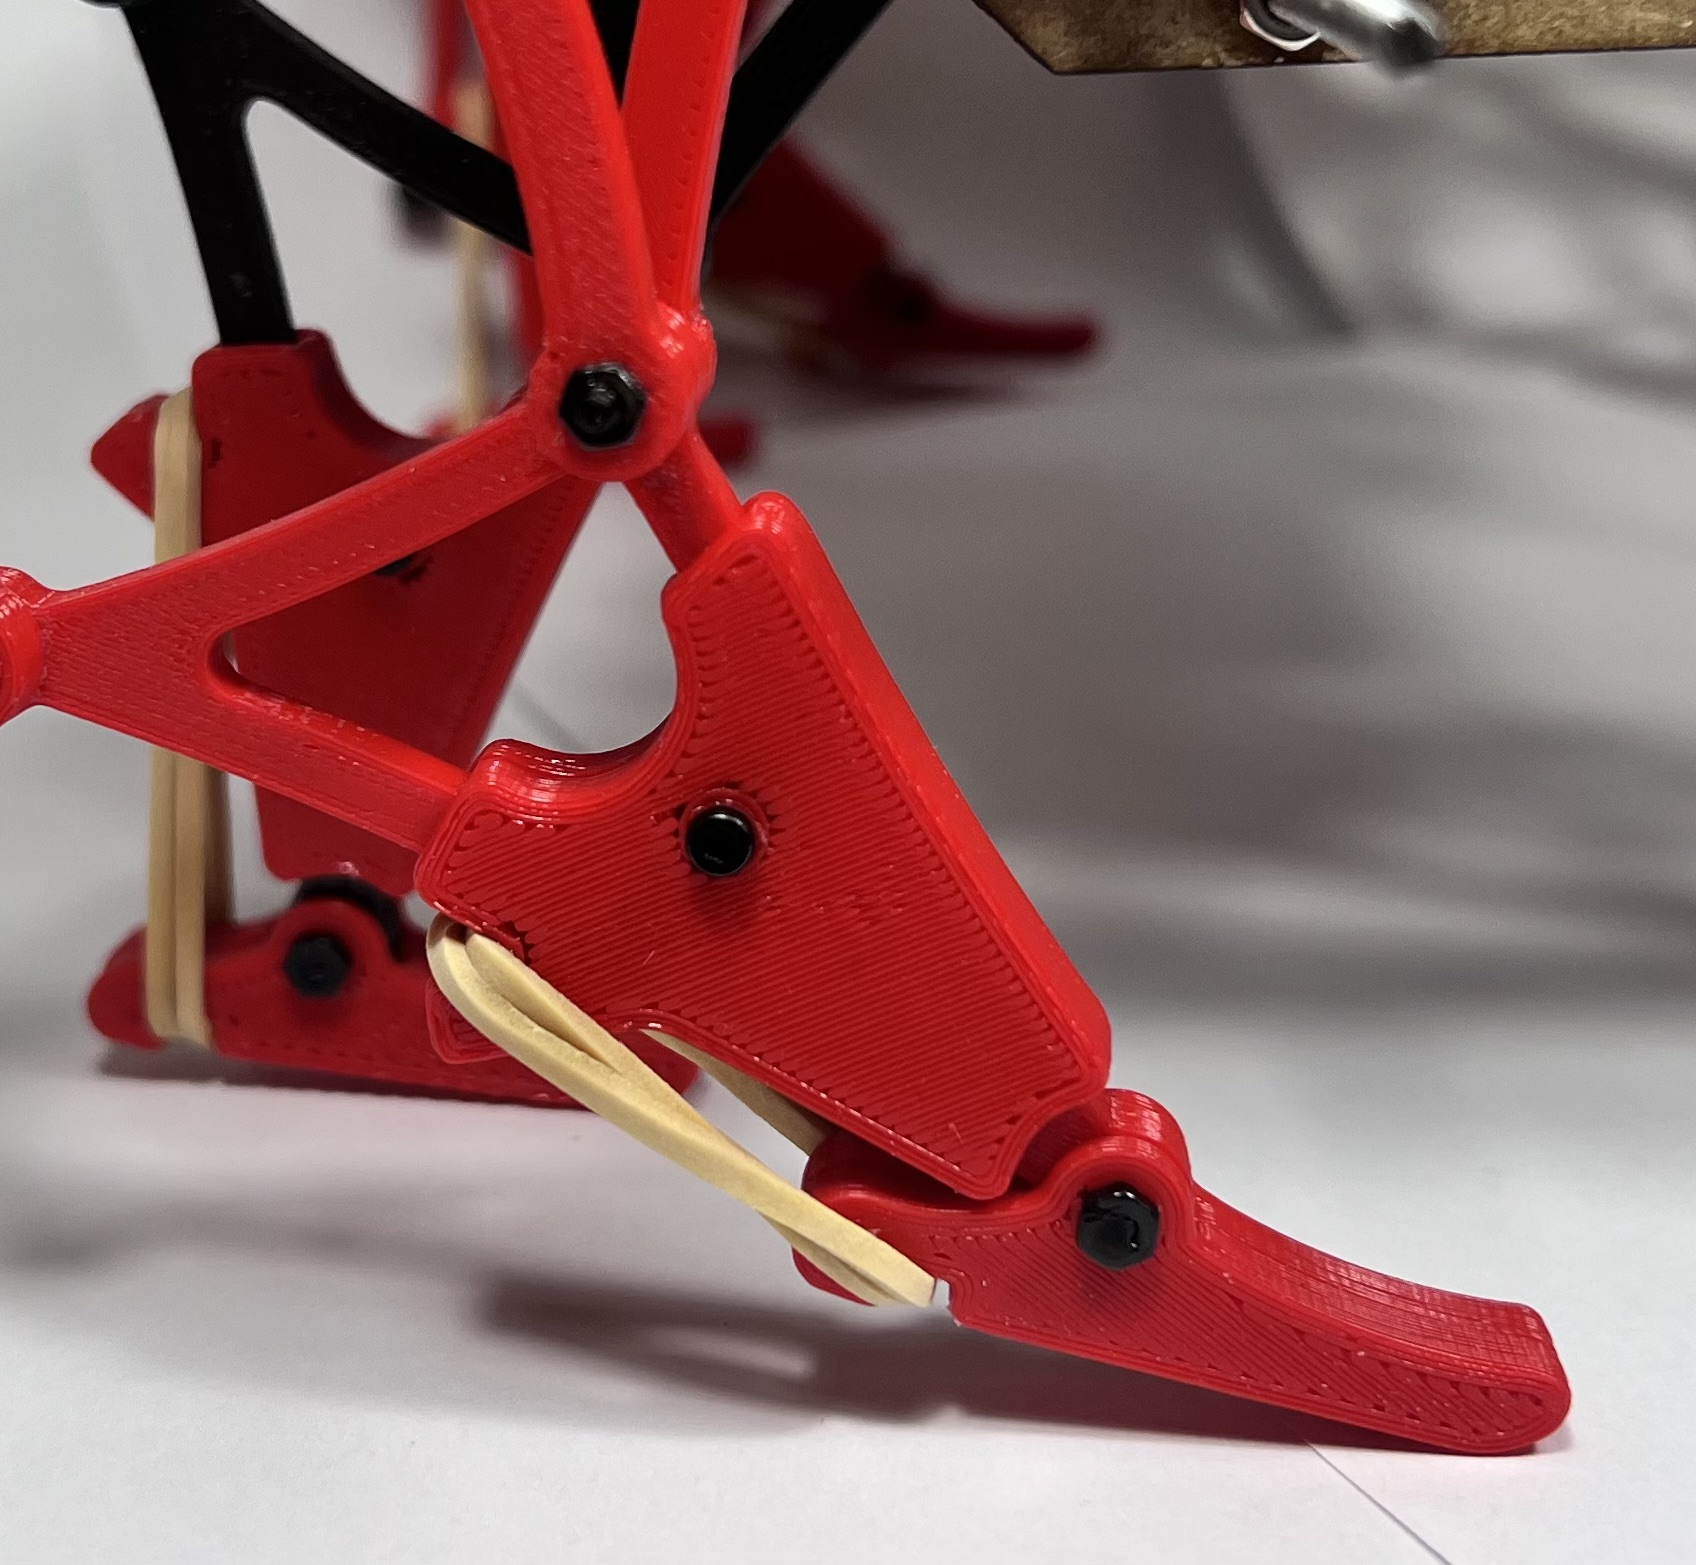
\includegraphics[width=1\linewidth]{images/Feet_assembly.jpeg}
    \caption{Acutated feet assembly}
    \label{fig:feet}
\end{figure}
\\ \\
One trade-off with this design is a reduction in backward walking speed, as the boot and foot are not symmetrical. Both parts are 3D-printed using PLA filament. To ensure a proper fit between the components, an inner wall tolerance of 0.25mm was used.
\subsection{Electronics}

\subsubsection{Microcontroller}
An Arduino Uno V3 is used as the microcontroller to manage all electronics of the robot. It distributes power from a 9V battery to the ultrasonic sensor, HM-10 Bluetooth module, and two DC motors. The onboard voltage regulator supplies 5V to components requiring lower voltage, such as the ultrasonic sensor and the HM-10 module. However, the motor shield provides the full 9V directly to the DC motors. The Arduino receives input from both the ultrasonic sensor and the Bluetooth module. Based on this data, it controls the movements of the robot by sending appropriate signals to the motor shield, which handles direction and speed control via PWM outputs. The entire circuit can be seen below in figure \ref{fig:Schematic}
\begin{figure} [!htb]
    \centering
    \includegraphics[width=1\linewidth]{images/Amandatory_exam_schem.png}
    \caption{Electronics schematic}
    \label{fig:Schematic}
\end{figure}
\subsubsection{Motor shield}
To simplify motor control and to help maintain a clean layout, a motor shield was used. The shield is based on the L298P dual H-bridge driver and mounts directly onto the Arduino, removing the need for additional wiring between the Arduino and a separate motor driver module. The L298P-based shield enables control of both the direction and speed of the motors. Directional control is achieved without manually constructing an H-bridge circuit, while speed is regulated using PWM (Pulse Width Modulation). This level of control was useful during testing of the robot, as it allowed us to evaluate how changes in mechanical design affected the required PWM values for minimal movement.
\\
\subsubsection{Ultra Sonic sensor (HC-SR04)}
To handle obstacle detection and prevent the robot from steering into walls, an ultrasonic sensor is used to detect nearby objects. The sensor is mounted to the baseplate using a custom bracket to ensure a forward-facing orientation. Depending on the model, the HC-SR04 ultrasonic sensor can have either three or four pins. In this implementation, a 3-pin version is used, which includes GND, VCC, and Signal. VCC and GND are connected to the Arduino’s 5V power rail and ground, respectively, while the Signal pin is connected to digital pin 7 on the Arduino. The ultrasonic sensor works by sending out a short burst of sound and measuring the time it takes for the echo to return. This data is then used to calculate the distance. 
\\
\subsubsection{Bluetooth interface (HM-10)}
One of the goals for this project was to be able to remote control the robot from a smartphone or other device, as such a communication device was needed to communication between the Arduino and external devices, a Bluetooth module was selected. After evaluating two common options, the HC-06 and the HM-10 we elected for the HM-10 due to its compatibility with IOS devices and support for Bluetooth Low Energy (BLE), which offers lower power consumption. The HM-10 module features four pins: VCC, GND, TXD (transmit), and RXD (receive). VCC and GND are connected to the Arduino’s 5V power rail and ground, respectively. Serial communication is handled via the TXD and RXD pins, which are connected to digital pins 4 and 5 on the Arduino.
\\ \\
Since the HM-10 operates on 3.3V logic levels, a voltage divider is used on the Arduino’s TX line to reduce the 5V signal to 3.3V. The RXD line from the module, which sends data to the Arduino, can be read directly without level shifting, as 3.3V is sufficient for a logic high on Arduino boards. The module recives data from a smartphone app, which controls the direction and speed of the robot.
\\
\subsubsection{DC-motor}
To drive the main axles on either side of the robot, DC motors were selected. Stepper and servo motors were considered, but not chosen, as the application did not need precision positioning. Instead, the focus was on sufficient torque to overcome friction. A lower RPM motor was chosen, rated at approximately 60 RPM. This slower motor provides higher torque. Alternatively, we could have used a higher RPM motor, though it would have been necessary to increase the gear ratio to achieve similar torque output. The DC motors are connected to the Arduino via the motor shield, allowing for both directional and speed control. Speed is regulated using PWM signals, enabling the system to adjust power to the motors.
\\
\subsubsection{Power}
To power both the Arduino and the DC motors, a 9V battery was used. This choice was made to provide higher voltage to the motors, improving their performance compared to lower-voltage alternatives. However, a drawback of the 9V battery is its capacity under load, resulting in frequent battery replacements during extended testing. An alternative setup using four 1.2V rechargeable batteries was tested, but ultimately rejected. This setup resulted in noticeably reduced motor performance and introduced a lot of additional weight. Both of those compounding factors led continuing to use of the 9V battery.
\\
\subsection{Software/Firmware}
This project involves two software components: the Arduino code, which controls the robot and reads data from the Bluetooth and ultrasonic sensors; and the IOS app, which sends signals to the Bluetooth module. Since app development is outside the scope of the course, only a brief overview of the UI and implementation will be provided. \\
\subsubsection{Arduino firmware}
The primary functions of the Arduino software is motor control, Bluetooth communication, and obstacle detection. Motor control is implemented via the motor shield, which enables control of motor direction, braking, and speed using PWM signals. Each motor is controlled using three pins: one for direction, one for braking, and one for speed (PWM). The direction and brake pins are digital and can be set to either HIGH or LOW to enable, disable, or reverse motor rotation. The speed pin uses PWM and accepts analog values between 0 and 255, enabling fine motor control. Appendix \ref{arduino_code} for source code
\\ \\
Commands are received via the HM-10 Bluetooth module. Upon receiving a command, the Arduino updates the relevant control pins for each motor accordingly. The system supports five directional commands: forward, backward, left, right, and stop. In addition to directional control, the Arduino can process speed commands that adjust the PWM output by increments of ±10, ±25 and ±50.
\\ \\
Obstacle detection is handled using the HC-SR04 ultrasonic sensor, which measures the distance to objects in front of the robot. If the detected distance falls below a defined threshold, the Arduino engages the motor brakes to prevent collisions. In this state, only speed, turn or reverse commands are accepted, ensuring that the robot avoids driving into obstacles.
\\
\subsubsection{IOS-app}
\begin{figure}
    \centering
    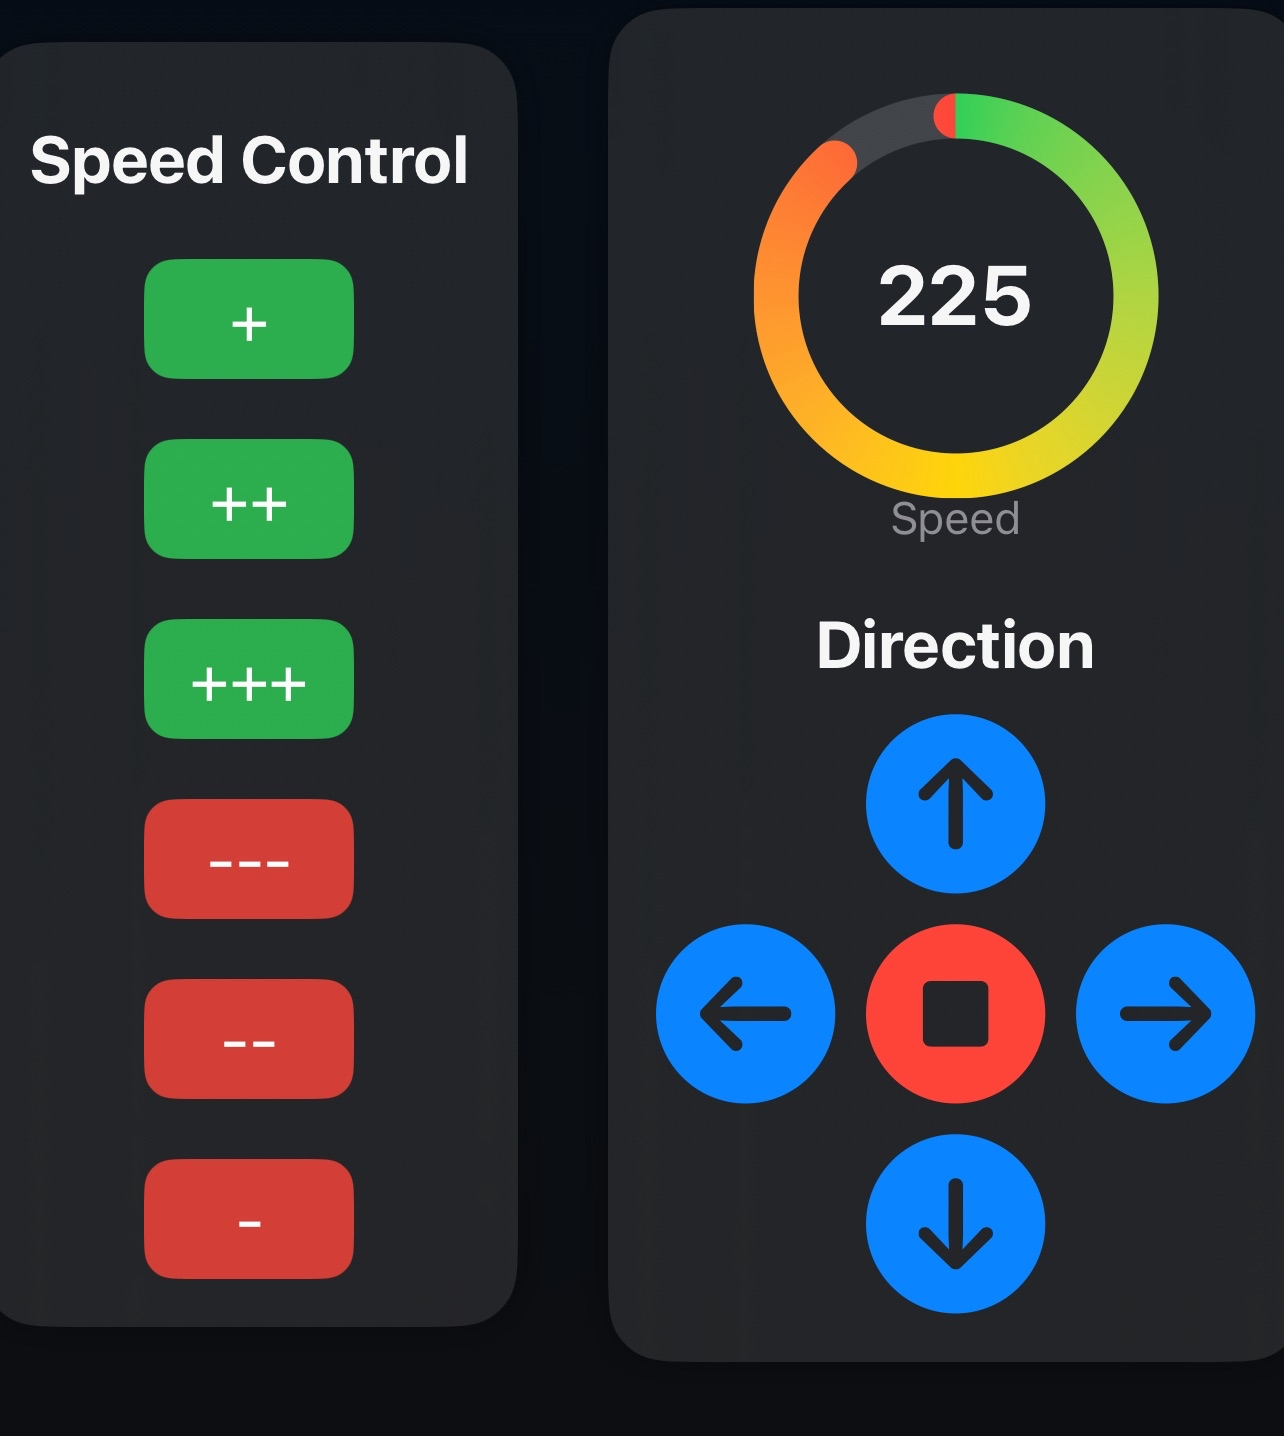
\includegraphics[width=1\linewidth]{images/IOS_app_interface.png}
    \caption{Interface of the app, with a PWM setting at 225}
    \label{fig:app_interface}
\end{figure}
The IOS app (see appendix: \ref{swift_code}, for source code), developed in Swift, connects to the HM-10 Bluetooth module on startup and automatically attempts to reconnect if the connection is lost. It features five directional buttons (forward, backward, left, right, stop) and six speed adjustment buttons (±10, ±25, ±50). A speedometer displays the current PWM value. When a button is pressed, the app sends the corresponding command to the Arduino via Bluetooth. The app interface is shown in Figure \ref{fig:app_interface}.
\section{Results/Analysis}
%Did it work properly? What kind of tests did you run to test your prototype? Could you provide some data that shows the performance of the prototype (speed, success rate, etc.)? Please, try to do some tests to show in a graph/table and give quantitative facts. It is not enough to build a device that works, you should test it properly. If does not work, try to test why it fails or test subsystems.
The robot, was originally made with a single set of legs on either side, by that point it was able to wobble around, propelling itself forward in a less than confident way. As the project continued and iterated upon, we added another set of legs on either side, making the robot move in a much more confident fashion. The addition of actuated feet further enhanced its mobility, allowing it to traverse soft surfaces like beds and sofas, as well as uneven and slippery terrain such as grass. During testing we found that the robot was leaning to one side when walking, this was somewhat alleviated by the actuated feet, and replacing one of the leg assemblies. Using the IOS app to control the robot, made the testing process very enjoyable, as the connection between the app and the robot is very responsive. Described below are the findings from our tests based on the requirements proposed earlier. \\
\subsubsection{Scaling}
The robot started of with four legs and was able to walk. When we added four more we could do it by changing the length of the beams and creating a set more, proving that the robot is scalable.
\\
\subsubsection{Bluetooth control}
The bluetooth app works and the robot reacts very quickly when pressing a button.
\\
\subsubsection{Motion}
Several tests have been performed, and the results can be seen in table \ref{tab:speed_test}. The same tests were performed both before and after the addition of actuated feet to see the performance difference. The results shows the speed in seconds how fast it can walk one meter. From the results we observe that the robot was able to walk faster after we added the feet, expect when it walks backwards. \\
Besides walking faster, the robot also walked in a more straight line. While before the actuated feet, we had to do the  tests multiple times as the robot walked off to the side and therefore didn't complete the test. 
\\
\begin{table}[!ht]
    \centering
    \begin{tabular}{|l|l|l|}
    \hline
        Test (speed) & Before feet: seconds & After feet: seconds \\ \hline
        Walking normally (255) & 5,53 & 4,87 \\ \hline
        Walking normally (175) & 7,03 & 6,67 \\ \hline
        Walking backwards (255) & 5,56 & 7,29 \\ \hline
        Walking on grass (255) & 18,88 & 14,78 \\ \hline
    \end{tabular}
    \caption{Results for testing speed}
    \label{tab:speed_test}
\end{table}
\subsubsection{Obstacle detection}
The robot would stop within 16 cm of a wall and is unable to walk forwards, only accepting commands for turning and walking backwards. 

\section{Discussion}
%What are the strengths and shortcomings of your device? Did it match the requirements? How would you improve/develop it further, if you had time? If you had to produce your device in a factory for mass production, what would you modify?
The robot is able to be remote controlled via the IOS app and avoids user error with obstacle detection via the ultrasonic sensor. With the addition of actuated feet, the robots performance was further improved enabling it to walk on rougher and more uneven surfaces. One major issue in regards to the robot is the difficulty in assembly, as one of the original goals of the project was to reduce weight, the overall footprint of the robot is relatively small. This results in the usage of m2 screws for assembly of the legs, resulting in finicky and frustrating assembly. Even given the relatively small footprint, friction is still the primary concern, and the point that could be improved the most. In a future iteration of the project, the usage of bearing would further decrease friction, perhaps enabling us to reduce the gear ratio, to increase speed. In addition, print-in-place joints for 3d-print manufacturing could be an interesting solution for leg assembly, as the entire leg would be printed as single object, something only enabled by usage of 3d-printing. \\ \\ For mass production the highest priority would be to ease the assembly of the legs, as such the aforementioned usage of print in place joints could be used to print the legs as a single object. To coalesce the electronics on the base and remove the breadboard, one could also develop a PCB to connect the different devices, in this case we could forego the expensive motor shield and instead use a motor driver, soldered into the pcb. This approach would be cheaper, while still eleminating wires.
%What are the strengths and shortcomings of your device? Did it match the requirements? How would you improve/develop it further, if you had time? If you had to produce your device in a factory for mass production, what would you modify?

\nocite{*}
\printbibliography
%You can add references, but they are not needed. (All the parts used in your project should be documented in the annexes.)
\clearpage
\onecolumn  
\appendices
\section{Video showcase}
\label{showcase}
Link to Video: \href{https://youtu.be/3B_pobduNls}{https://youtu.be/3B_pobduNls} 
\section{IOS-app code}
\label{swift_code}
\begin{lstlisting}[language=c++]
import SwiftUI
import CoreBluetooth

struct ContentView: View {
    @StateObject private var bluetoothManager = BluetoothManager()
    @State private var speed: Int = 0

    var body: some View {
        ZStack {
            LinearGradient(gradient: Gradient(colors: [.blue.opacity(0.1), 
            .gray.opacity(0.1)]), startPoint: .top, endPoint: .bottom)
                .ignoresSafeArea()

            HStack(spacing: 30) {
                VStack(spacing: 20) {
                    Text("Speed Control")
                        .font(.title2)
                        .bold()
                        .padding(.top, 10)

                    ForEach([("+", 10, "z"), ("++", 25, "x"), ("+++", 50, "c"),
                             ("---", -50, "v"),
                             ("--", -25, "b"), ("-", -10, "n")], id: \.0)
                             { label, change, char in
                        Button(action: {
                            adjustSpeed(by: change, send: char)
                        }) {
                            Text(label)
                                .font(.title2)
                                .frame(width: 70, height: 40)
                                .background(change > 0 ? Color.green.opacity(0.8) : 
                                Color.red.opacity(0.8))
                                .foregroundColor(.white)
                                .cornerRadius(10)
                        }
                    }



                }
                .padding()
                .background(.ultraThinMaterial)
                .cornerRadius(20)
                .shadow(radius: 5)

                VStack(spacing: 10) {
                    VStack(spacing: 5) {
                        ZStack {
                            Circle()
                                .stroke(Color.gray.opacity(0.3), lineWidth: 15)
                                .frame(width: 120, height: 120)

                            Circle()
                                .trim(from: 0.0, to: CGFloat(speed) / 255)
                                .stroke(
                                    AngularGradient
                                    (gradient: Gradient(colors: [.green, .yellow, .red])
                                    , center: .center),
                                    style: StrokeStyle(lineWidth: 15, lineCap: .round)
                                )
                                .rotationEffect(.degrees(-90))
                                .frame(width: 120, height: 120)

                            Text("\(speed)")
                                .font(.title)
                                .bold()
                        }

                        Text("Speed")
                            .font(.subheadline)
                            .foregroundColor(.gray)
                    }
                    .padding(.top, 20)
                    
                    Text("Direction")
                        .font(.title2)
                        .bold()
                        .padding(.top, 10)

                    HStack(spacing: 25) {
                        Spacer()

                        Button(action: {
                            bluetoothManager.sendData("f")
                        }) {
                            Image(systemName: "arrow.up.circle.fill")
                                .resizable()
                                .frame(width: 60, height: 60)
                                .foregroundColor(.blue)
                        }

                        Spacer()
                    }

                    HStack(spacing: 10) {
                        Button(action: {
                            bluetoothManager.sendData("l")
                        }) {
                            Image(systemName: "arrow.left.circle.fill")
                                .resizable()
                                .frame(width: 60, height: 60)
                                .foregroundColor(.blue)
                        }

                        Button(action: {
                            bluetoothManager.sendData("s")
                        }) {
                            Image(systemName: "stop.circle.fill")
                                .resizable()
                                .frame(width: 60, height: 60)
                                .foregroundColor(.red)
                        }

                        Button(action: {
                            bluetoothManager.sendData("r")
                        }) {
                            Image(systemName: "arrow.right.circle.fill")
                                .resizable()
                                .frame(width: 60, height: 60)
                                .foregroundColor(.blue)
                        }
                    }

                    HStack(spacing: 25) {
                        Spacer()
                        Button(action: {
                            bluetoothManager.sendData("b")
                        }) {
                            Image(systemName: "arrow.down.circle.fill")
                                .resizable()
                                .frame(width: 60, height: 60)
                                .foregroundColor(.blue)
                        }
                        Spacer()
                    }
                }
                .padding()
                .background(.ultraThinMaterial)
                .cornerRadius(20)
                .shadow(radius: 5)
            }
            .padding()
        }
        .onAppear {
            bluetoothManager.startScan()
        }
        .onChange(of: bluetoothManager.isConnected) { connected in
            if connected {
                speed = 0
            }
        }
    }

    func adjustSpeed(by amount: Int, send character: String) {
        speed = max(0, min(255, speed + amount))
        bluetoothManager.sendData(character)
    }
}
class BluetoothManager: NSObject, ObservableObject,
CBCentralManagerDelegate, CBPeripheralDelegate {
    var centralManager: CBCentralManager!
    var hm10Peripheral: CBPeripheral!
    let hm10ServiceUUID = CBUUID(string: "FFE0")
    let hm10CharacteristicUUID = CBUUID(string: "FFE1")
    var txCharacteristic: CBCharacteristic?
    @Published var isConnected: Bool = false

    override init() {
        super.init()
        centralManager = CBCentralManager(delegate: self, queue: nil)
    }

    func centralManagerDidUpdateState(_ central: CBCentralManager) {
        if central.state == .poweredOn {
            startScan()
        } else {
            print("Bluetooth not available")
        }
    }

    func startScan() {
        print("Starting scan...")
        centralManager.
        scanForPeripherals(withServices: [hm10ServiceUUID], options: nil)
    }


    func centralManager(_ central: CBCentralManager,
    didDiscover peripheral: CBPeripheral,
    advertisementData: [String : Any], rssi RSSI: NSNumber) {
        print("Discovered \(peripheral.name ?? "Unknown")")
        hm10Peripheral = peripheral
        hm10Peripheral.delegate = self
        centralManager.stopScan()
        centralManager.connect(hm10Peripheral)
    }

    func centralManager(_ central: CBCentralManager,
    didConnect peripheral: CBPeripheral) {
        print("Connected to \(peripheral.name ?? "Unknown")")
        isConnected = true
        peripheral.discoverServices([hm10ServiceUUID])
    }

    func peripheral(_ peripheral: CBPeripheral,
    didDiscoverServices error: Error?) {
        if let services = peripheral.services {
            for service in services {
                peripheral.discoverCharacteristics([hm10CharacteristicUUID], for: service)
            }
        }
    }

    func peripheral(_ peripheral: CBPeripheral,
    didDiscoverCharacteristicsFor service: CBService, error: Error?) {
        if let characteristics = service.characteristics {
            for characteristic in characteristics {
                if characteristic.uuid == hm10CharacteristicUUID {
                    txCharacteristic = characteristic
                    peripheral.setNotifyValue(true, for: characteristic)
                    print("Characteristic connected")
                }
            }
        }
    }

    func sendData(_ message: String) {
        guard let txCharacteristic = txCharacteristic else { return }
        if let data = message.data(using: .utf8) {
            hm10Peripheral.
            writeValue(data, for: txCharacteristic, type: .withoutResponse)
            print("Sent: \(message)")
        }
    }
    
    func centralManager(_ central: CBCentralManager,
    didDisconnectPeripheral peripheral: CBPeripheral, error: (any Error)?) {
        print("Disconnected. Reconnect to try again.")
        startScan()
    }

}



\end{lstlisting}
\section{Arduino code}
\label{arduino_code}
\begin{lstlisting}[language=c++]
#include <SoftwareSerial.h>
SoftwareSerial BT(4,5);
char val; //value to receieve data from the serial port
char moveVal;
char speedVal;
char moveChars[] = {'l', 'r', 'f', 'b', 's'};
int speed = 0;
const int threshold = 20;
const int pingPin = 7;

void setup() {
  
  BT.begin(9600); //Bluetooth serial communications at 9600
  Serial.begin(4800); // Serial communication for logging to terminal
  if( BT.available() ) // check if there is data to read
  {
    val = BT.read(); // read the data into our value variable
  }

  //Setup Channel A
  pinMode(12, OUTPUT); //Initiates Motor Channel A pin
  pinMode(9, OUTPUT); //Initiates Brake Channel A pin

  //Setup Channel B
  pinMode(13, OUTPUT); //Initiates Motor Channel A pin
  pinMode(8, OUTPUT);  //Initiates Brake Channel A pin
  
}


void loop(){

  if( BT.available() ) // check if there is data to read
  {
    val = BT.read(); // read the data into our value variable
    handleVal(val);
  }

  if (measureDistance() < threshold && moveVal == 'f'){
    moveVal = ' ';
    digitalWrite(9, HIGH);  
    digitalWrite(8, HIGH);  
  }

  if (speedVal == 'z'){ // +
    changeSpeed(10);
  }
  if (speedVal == 'x'){ // ++
    changeSpeed(25);
  }
  if (speedVal == 'c'){ // +++
    changeSpeed(50);
  }
  if (speedVal == 'v'){ // ---
    changeSpeed(-50);
  }
  if (speedVal == 'b'){ // --
    changeSpeed(-25);
  }
  if (speedVal == 'n'){ // -
    changeSpeed(-10);
  }

  if (moveVal == 'f') { // Forward
    digitalWrite(12, HIGH); 
    digitalWrite(9, LOW);  
    analogWrite(3, speed);   

    digitalWrite(13, LOW);  
    digitalWrite(8, LOW);   
    analogWrite(11, speed);    
  }
  if (moveVal == 'b') { // Backward 
    digitalWrite(12, LOW); 
    digitalWrite(9, LOW);   
    analogWrite(3, speed);   

    digitalWrite(13, HIGH);  
    digitalWrite(8, LOW);   
    analogWrite(11, speed);    


  }

  if (moveVal == 'r') { // right
    digitalWrite(12, HIGH); 
    digitalWrite(9, LOW);   
    analogWrite(3, speed);   

    digitalWrite(13, HIGH);  
    digitalWrite(8, LOW);   
    analogWrite(11, speed);    
  }

  if (moveVal == 'l') { // left
    digitalWrite(12, LOW); 
    digitalWrite(9, LOW);   
    analogWrite(3, speed);   

    digitalWrite(13, LOW);  
    digitalWrite(8, LOW);   
    analogWrite(11, speed);    

  }
  if (moveVal == 's') { // stop
    digitalWrite(9, HIGH);  
    digitalWrite(8, HIGH);  
  }
  

  delay(100);

  
}

void handleVal(char x){
  // If the value is a direction assign it to the moveval, 
  // which will not be wiped after a loop.
  // Otherwise assign it as the speedval, which will be wiped.
  for (int i = 0; i < sizeof(moveChars); i++) {
    if (x == moveChars[i]) {
      moveVal = val;
      return;
    }
  }
  speedVal = val;
}

// Wrap around function, so the pwm value cannot exceed 255, and go below 0
void changeSpeed(int x){
  if((speed + x) >= 255){
    speed = 255;
    speedVal = ' ';
    return;
  } 
  if ((speed + x) <= -1) {
    speed = 0;
    speedVal = ' ';
    return;
  }
  speedVal = ' ';
  speed = speed + x;
}


int measureDistance(){
  long duration, cm;

  // Send out trigger pulse, to measure afterwards
  pinMode(pingPin, OUTPUT);
  digitalWrite(pingPin, LOW);
  delayMicroseconds(2);
  digitalWrite(pingPin, HIGH);
  delayMicroseconds(4);
  digitalWrite(pingPin, LOW);

  // Measure the duration of the pulse
  pinMode(pingPin, INPUT);
  duration = pulseIn(pingPin, HIGH);

  // convert the time into a distance
  cm = duration / 29 / 2;

  Serial.print(cm);
  Serial.print("cm");
  Serial.println();

  return cm;
}
\end{lstlisting}

\section{Bill of Materials}
\begin{table}[!ht]
    \centering
    \begin{tabular}{|l|l|l|l|}
    \hline
        Component & Quantity & Cost per unit & Subtotal \\ \hline
        Arduino R3 & 1 & kr 236,25 & kr 236,25 \\ \hline
        Heemol L298P Shield R3  & 1 & kr 112 & kr 112 \\\hline
        DSD TECH HM-10 & 1 & 86,16 & 86,16  \\\hline
        DC Motor & 2 & kr 13,05 & kr 26,10 \\ \hline
        Breadboard & 1 & kr 37,95 & kr 37,95 \\ \hline
        Parts for legs & 4 & kr 0,26 & kr 1,04 \\ \hline
        Spur Gear (6 teeth) & 4 & kr 0,03 & kr 0,12 \\ \hline
        Spur Gear (18 teeth) * & 8 & ~ & kr 0,00 \\ \hline
        motorClamp\_left & 1 & kr 0,20 & kr 0,20 \\ \hline
        motorClamp\_right & 1 & kr 0,20 & kr 0,20 \\ \hline
        Gear mounting plate * & 2 & ~ & kr 0,00 \\ \hline
        Baseplate * & 1 & ~ & kr 0,00 \\ \hline
        BEAM 1X1 & 4 & kr 0,34 & kr 1,36 \\ \hline
        CROSS AXLE 6M & 2 & kr 0,91 & kr 1,82 \\ \hline
        Left\_L\_bracket & 1 & kr 0,25 & kr 0,25 \\ \hline
        Right\_L\_bracket & 1 & kr 0,25 & kr 0,25 \\ \hline
        feet\_top & 8 & kr 0,05 & kr 0,40 \\ \hline
        feet\_bottom & 8 & kr 0,04 & kr 0,32 \\ \hline
        hc-sc04  & 1 & kr 0,26 & kr 0,26 \\ \hline
        Rubber bands & 8 & kr 1,27 & kr 10,19 \\ \hline
         &  & Total cost & \underline{kr 514,87}\\ \hline
    \end{tabular}
\end{table}
* we have been unable find the cost of lasercutting

\section{Technical drawings}
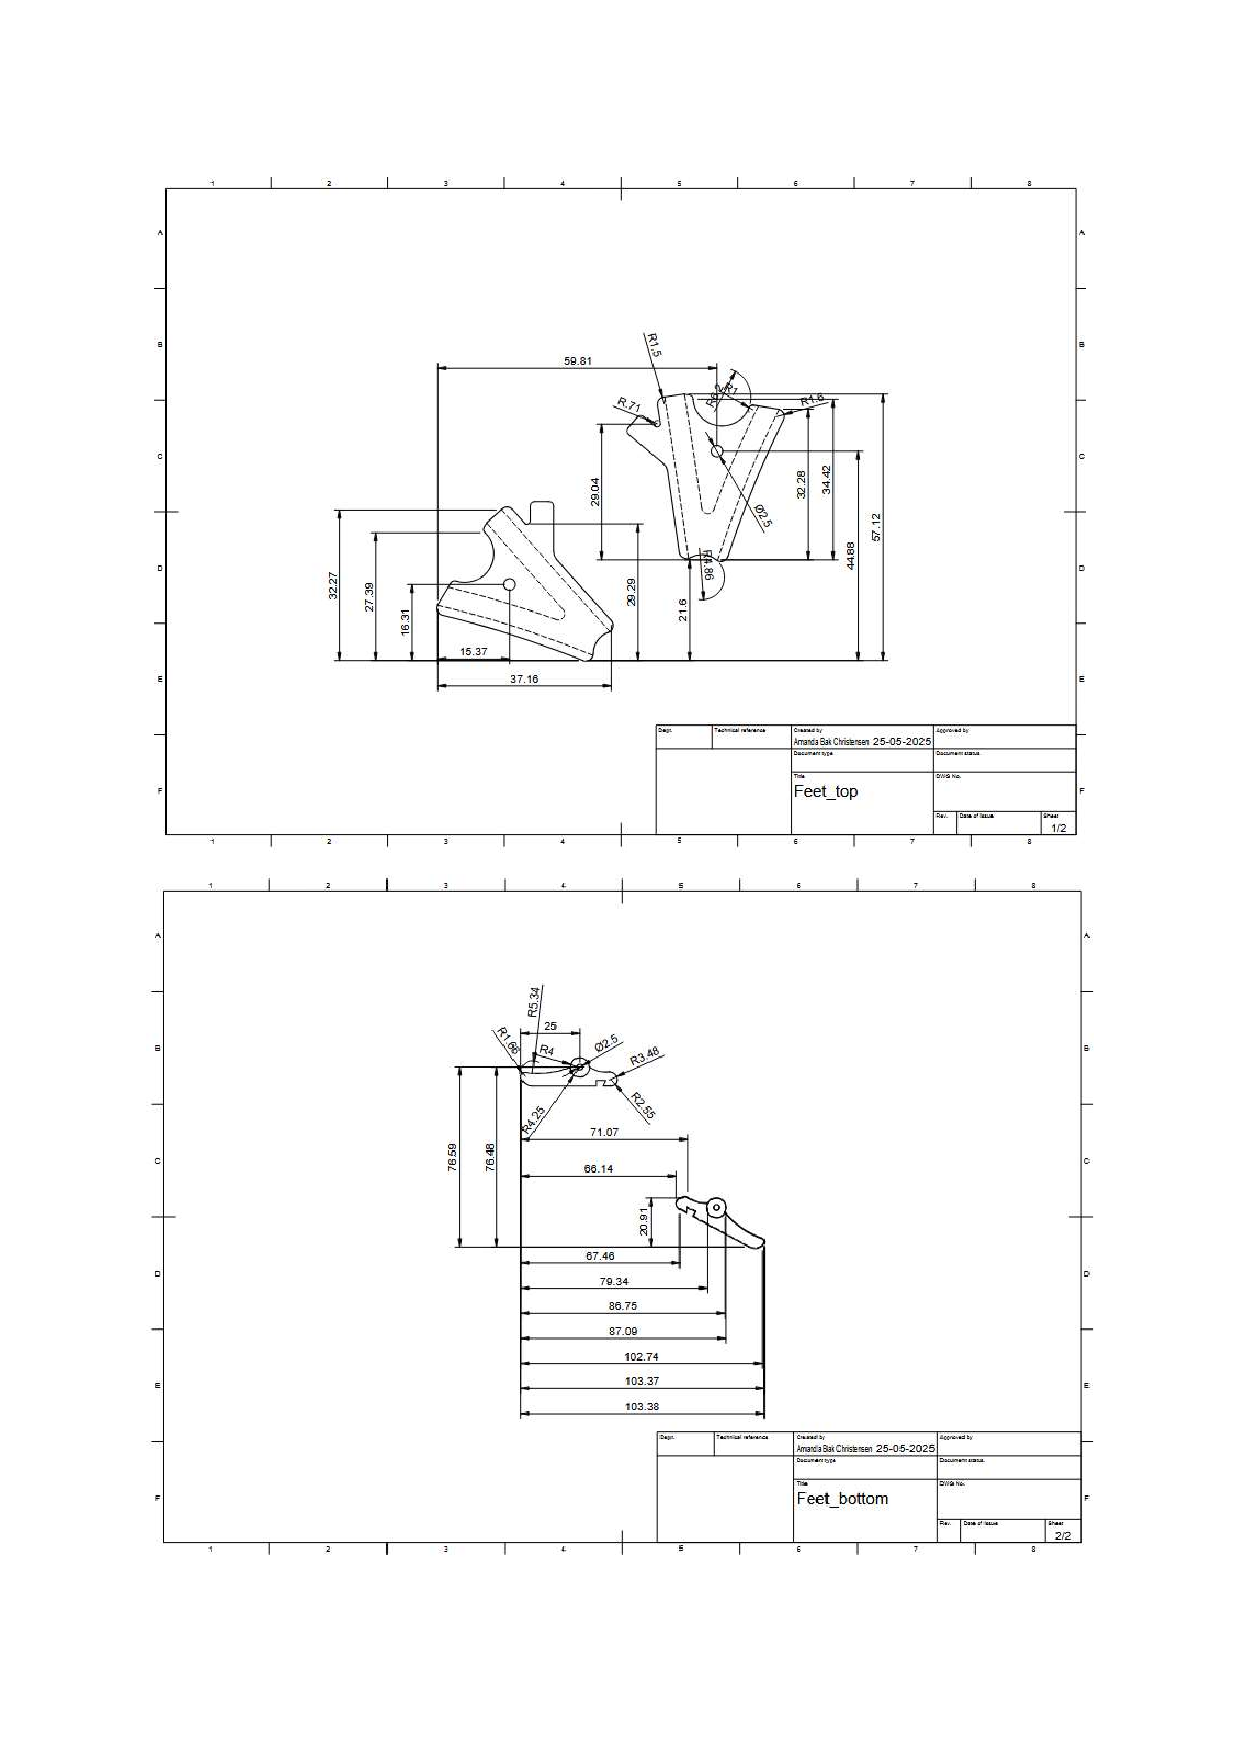
\includepdf[pages=-]{Appendix/Technical drawings}
\subsection{Part wise assembly}
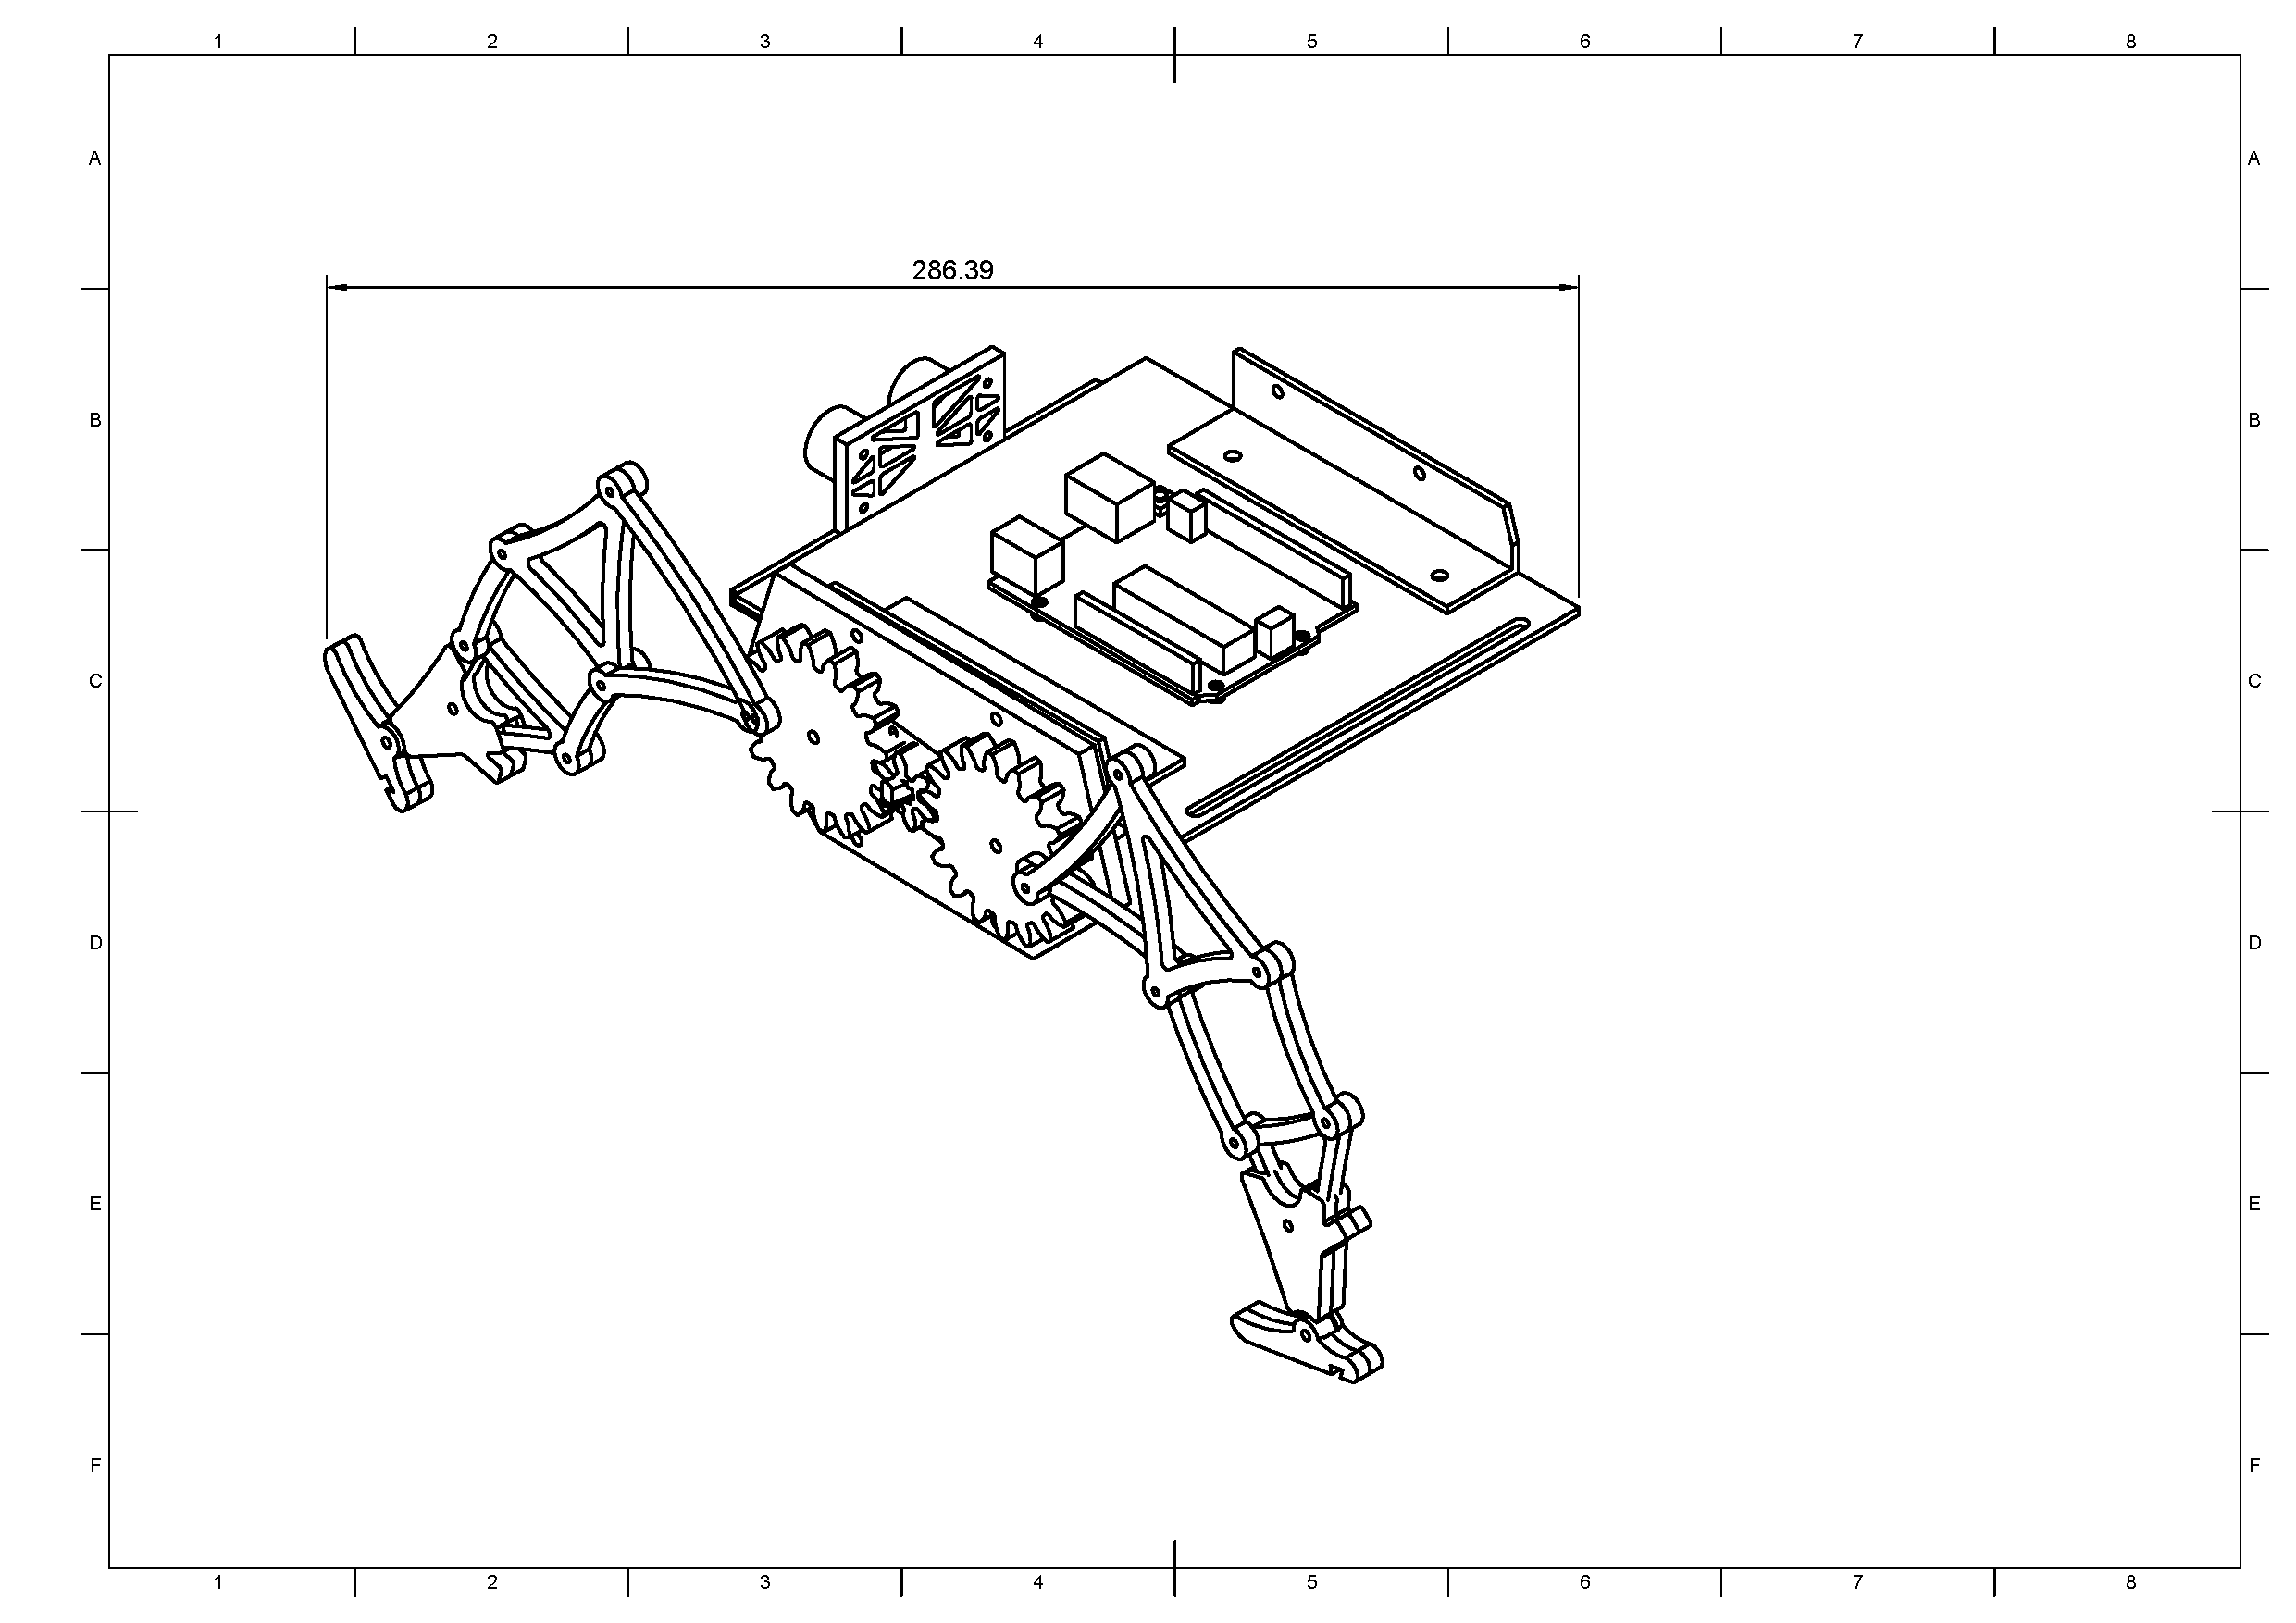
\includepdf[pages=-]{Appendix/Part_assembly v1}
\section{Electrical schematics}
\includegraphics[scale = 1.0]{Appendix/Amandatory_exam_schem.png}


% An example of a floating figure using the graphicx package.
% Note that \label must occur AFTER (or within) \caption.
% For figures, \caption should occur after the \includegraphics.
% Note that IEEEtran v1.7 and later has special internal code that
% is designed to preserve the operation of \label within \caption
% even when the captionsoff option is in effect. However, because
% of issues like this, it may be the safest practice to put all your
% \label just after \caption rather than within \caption{}.
%
% Reminder: the "draftcls" or "draftclsnofoot", not "draft", class
% option should be used if it is desired that the figures are to be
% displayed while in draft mode.
%
%\begin{figure}[!t]
%\centering
%\includegraphics[width=2.5in]{myfigure}
% where an .eps filename suffix will be assumed under latex, 
% and a .pdf suffix will be assumed for pdflatex; or what has been declared
% via \DeclareGraphicsExtensions.
%\caption{Simulation results for the network.}
%\label{fig_sim}
%\end{figure}

% Note that IEEE typically puts floats only at the top, even when this
% results in a large percentage of a column being occupied by floats.


% An example of a double column floating figure using two subfigures.
% (The subfig.sty package must be loaded for this to work.)
% The subfigure \label commands are set within each subfloat command,
% and the \label for the overall figure must come after \caption.
% \hfil is used as a separator to get equal spacing.
% Watch out that the combined width of all the subfigures on a 
% line do not exceed the text width or a line break will occur.
%
%\begin{figure*}[!t]
%\centering
%\subfloat[Case I]{\includegraphics[width=2.5in]{box}%
%\label{fig_first_case}}
%\hfil
%\subfloat[Case II]{\includegraphics[width=2.5in]{box}%
%\label{fig_second_case}}
%\caption{Simulation results for the network.}
%\label{fig_sim}
%\end{figure*}
%
% Note that often IEEE papers with subfigures do not employ subfigure
% captions (using the optional argument to \subfloat[]), but instead will
% reference/describe all of them (a), (b), etc., within the main caption.
% Be aware that for subfig.sty to generate the (a), (b), etc., subfigure
% labels, the optional argument to \subfloat must be present. If a
% subcaption is not desired, just leave its contents blank,
% e.g., \subfloat[].


% An example of a floating table. Note that, for IEEE style tables, the
% \caption command should come BEFORE the table and, given that table
% captions serve much like titles, are usually capitalized except for words
% such as a, an, and, as, at, but, by, for, in, nor, of, on, or, the, to
% and up, which are usually not capitalized unless they are the first or
% last word of the caption. Table text will default to \footnotesize as
% IEEE normally uses this smaller font for tables.
% The \label must come after \caption as always.
%
%\begin{table}[!t]
%% increase table row spacing, adjust to taste
%\renewcommand{\arraystretch}{1.3}
% if using array.sty, it might be a good idea to tweak the value of
% \extrarowheight as needed to properly center the text within the cells
%\caption{An Example of a Table}
%\label{table_example}
%\centering
%% Some packages, such as MDW tools, offer better commands for making tables
%% than the plain LaTeX2e tabular which is used here.
%\begin{tabular}{|c||c|}
%\hline
%One & Two\\
%\hline
%Three & Four\\
%\hline
%\end{tabular}
%\end{table}


% Note that the IEEE does not put floats in the very first column
% - or typically anywhere on the first page for that matter. Also,
% in-text middle ("here") positioning is typically not used, but it
% is allowed and encouraged for Computer Society conferences (but
% not Computer Society journals). Most IEEE journals/conferences use
% top floats exclusively. 
% Note that, LaTeX2e, unlike IEEE journals/conferences, places
% footnotes above bottom floats. This can be corrected via the
% \fnbelowfloat command of the stfloats package.






% trigger a \newpage just before the given reference
% number - used to balance the columns on the last page
% adjust value as needed - may need to be readjusted if
% the document is modified later
%\IEEEtriggeratref{8}
% The "triggered" command can be changed if desired:
%\IEEEtriggercmd{\enlargethispage{-5in}}

% references section

% can use a bibliography generated by BibTeX as a .bbl file
% BibTeX documentation can be easily obtained at:
% http://www.ctan.org/tex-archive/biblio/bibtex/contrib/doc/
% The IEEEtran BibTeX style support page is at:
% http://www.michaelshell.org/tex/ieeetran/bibtex/

% argument is your BibTeX string definitions and bibliography database(s)
%\bibliography{IEEEabrv,../bib/paper}
%
% <OR> manually copy in the resultant .bbl file
% set second argument of \begin to the number of references
% (used to reserve space for the reference number labels box)





% that's all folks
\end{document}


